\documentclass[authordate, empirical]{jote-new-article}

\usepackage{caption}

\usepackage{tabularx}

\usepackage{graphicx}

\usepackage{hyperref}


\usepackage[backend=biber,style=apa]{biblatex}

\addbibresource{bibliography.bib}

\jotetitle{Cognitive Functions, Mood and Sleep Quality after Two Months of Intermittent Fasting}
\keywordsabstract{intermittent fasting, cognitive functions, mood, sleep quality, mental health}
\abstracttext{Intermittent fasting is being popularized as a method beneficial not only for weight loss, but also for overall psychological functioning and well-being. However, there is only a handful of studies examining the latter claims. The aim of this open-label study was to contribute to the understanding of the relationship between fasting-based diets, and cognitive functions and other mental health factors such as mood and sleep quality. The research was conducted on a sample of 105 healthy volunteers who were placed in either the experimental (fasting) group (\emph{n} = 76) or the control (no change in diet regimen) group (\emph{n} = 29). For a period of 2 months, the experimental group adhered to a time-restricted eating (TRE) form of intermittent fasting: Participants were instructed to fast from eating or drinking for 16 hours per day. Participants in the control group did not adhere to any specific dietary regimen. Cognitive functioning (attention, memory, working memory and executive functions), as well as sleep quality and several mood dimensions (anxiety, depression, fatigue, hostility, friendliness, cheerfulness, concentration, energy) were measured across three time points: Prior to the beginning of the study, and one month and two months later, respectively. Results showed no significant group x time point interactions on any of the measures. In conclusion, the results of this study do not corroborate the notion that TRE regimen significantly influences cognitive functions, mood or sleep of healthy individuals. While fasting-based diets successfully regulate weight, the claims regarding their beneficial effect on psychological functioning in non-clinical populations are yet to be proven. }
\runningauthor{Hromatko et al.}
\jname{Journal of Trial \& Error}
\jyear{2024}
\paperdoi{10.36850/e71f-5cff}
\paperreceived{July 4, 2023}
\author[1]{\mbox{Maja Batorek\orcid{0000-0002-2807-4226}}}
\affil[1]{University of Zagreb}
\author[2]{\mbox{Ivana Hromatko\orcid{0000-0002-3837-1929}}}
\affil[2]{University of Zagreb, Faculty of Humanities and Social Sciences, Dept. of Psychology}
\corremail{\href{mailto:ihromatko@ffzg.hr}{ihromatko@ffzg.hr}}
\corraddress{University of Zagreb, Faculty of Humanities and Social Sciences, Dept. of Psychology}
\runningauthor{Hromatko \& Batorek}
\paperaccepted{April 11, 2024}
\paperpublished{August 11, 2024}
\paperpublisheddate{2024-06-30}
\jwebsite{https://journal.trialanderror.org}

\begin{filecontents}{bibliography.bib}
	@article{undefined2017,
    title       = {the metabolic switch: {U}nderstanding and applying the health benefits of fasting},
    author      = {Anton, S. D., Moehl, K., Donahoo, W. T., Marosi, K., Lee, S. A., Mainous, A. G., Leeuwenburgh, C., \&, Mattson, M. P.},
    number      = {2},
    volume      = {26},
    url         = {https://doi.org/10.1002/oby.22065},
    doi         = {10.1002/oby.22065},
    date        = {2017},
    pages       = {254--268},
    journal     = {Obesity}
}


@article{Antoni2017,
    title       = {Effects of intermittent fasting on glucose and lipid metabolism. Proceedings of the Nutrition Society, 76(3},
    author      = {Antoni, R. and Johnston, K. L. and Collins, A. L. and Robertson, M. D.},
    url         = {https://doi.org/10.1017/s0029665116002986},
    doi         = {10.1017/s0029665116002986},
    date        = {2017},
    pages       = {361--368}
}


@article{Appleton2015,
    title       = {Distraction, not hunger, is associated with lower mood and lower perceived work performance on fast compared to non-fast days during intermittent fasting},
    author      = {Appleton, K. M. and Baker, S.},
    number      = {6},
    volume      = {20},
    url         = {https://doi.org/10.1177/1359105315573430},
    doi         = {10.1177/1359105315573430},
    date        = {2015},
    pages       = {702--711},
    journal     = {Journal of Health Psychology}
}


@article{Arnold2018,
    title       = {insulin resistance in type 2 diabetes and Alzheimer disease: concepts and conundrums},
    author      = {Arnold, S. E. and Arvanitakis, Z. and Macauley-Rambach, S. L. and Koenig, A. M. and Wang, H.-Y. and Ahima, R. S. and Craft, S. and Gandy, S. and Buettner, C. and Stoeckel, L. E. and Holtzman, D. M. and Nathan, D. M.},
    number      = {3},
    volume      = {14},
    url         = {https://doi.org/10.1038/nrneurol.2017.185},
    doi         = {10.1038/nrneurol.2017.185},
    date        = {2018},
    pages       = {168--181},
    journal     = {Nature Reviews Neurology}
}


@article{Arnoldussen2014,
    title       = {Obesity and dementia: {A}dipokines interact with the brain. European Neuropsychopharmacology, 24(12},
    author      = {Arnoldussen, I. A. and Kiliaan, A. J. and Gustafson, D. R.},
    url         = {https://doi.org/10.1016/j.euroneuro.2014.03.002},
    doi         = {10.1016/j.euroneuro.2014.03.002},
    date        = {2014}
}


@inbook{Axelrod2007,
    title       = {Nonrandomized interventional study designs (quasi-experimental designs},
    author      = {Axelrod, D. A. and Hayward, R.},
    editor      = {Penson, D.F. and Wei, J.T.},
    url         = {https://doi.org/10.1007/978-1-59745-230-4},
    doi         = {10.1007/978-1-59745-230-4},
    publisher   = {Humana Totowa},
    date        = {2007},
    pages       = {63--76},
    booktitle     = {Clinical Research Methods for Surgeons}
}


@article{Backhaus2002,
    title       = {Test--retest reliability and validity of the Pittsburgh Sleep Quality Index in primary insomnia. Journal of Psychosomatic Research, 53(3},
    author      = {Backhaus, J. and Junghanns, K. and Broocks, A. and Riemann, D. and Hohagen, F.},
    url         = {https://doi.org/10.1016/s0022-3999(02)00330-6},
    doi         = {10.1016/s0022-3999(02)00330-6},
    date        = {2002},
    pages       = {737--740}
}


@article{Barnosky2014,
    title       = {Intermittent fasting vs daily calorie restriction for type 2 diabetes prevention: a review of human findings. Translational Research, 164(4},
    author      = {Barnosky, A. R. and Hoddy, K. K. and Unterman, T. G. and Varady, K. A.},
    url         = {https://doi.org/10.1016/j.trsl.2014.05.013},
    doi         = {10.1016/j.trsl.2014.05.013},
    date        = {2014},
    pages       = {302--311}
}


@article{Bear2021,
    title       = {The microbiome-gut-brain axis and resilience to developing anxiety or depression under stress. Microorganisms, 9(4},
    author      = {Bear, T. and Dalziel, J. and Coad, J. and Roy, N. and Butts, C. and Gopal, P.},
    volume      = {723},
    url         = {https://doi.org/10.3390/microorganisms9040723},
    doi         = {10.3390/microorganisms9040723},
    date        = {2021},
    journal     = {Article}
}


@article{Bedrosian2017,
    title       = {Timing of light exposure affects mood and brain circuits. Translational Psychiatry, 7(1},
    author      = {Bedrosian, T. A. and Nelson, R. J.},
    url         = {https://doi.org/10.1038/tp.2016.262},
    doi         = {10.1038/tp.2016.262},
    date        = {2017},
    pages       = {1017-- 1017}
}


@article{Bekinschtein2014,
    author      = {Bekinschtein, P. and Cammarota, M. and Medina, J. H.},
    number      = {armacology, 76},
    url         = {https://doi.org/10.1016/j.neuropharm.2013.04.024},
    doi         = {10.1016/j.neuropharm.2013.04.024},
    date        = {2014},
    pages       = {677--683},
    journal     = {BDNF and memory}
}


@article{Benau2021,
    title       = {How does fasting affect cognition? An updated systematic review (2013-2020},
    author      = {Benau, E. M. and Makara, A. and Orloff, N. C. and Benner, E. and Serpell, L. and Timko, C. A.},
    number      = {4},
    volume      = {10},
    url         = {https://doi.org/10.1007/s13668-021-00370-4},
    doi         = {10.1007/s13668-021-00370-4},
    date        = {2021},
    pages       = {376--390},
    journal     = {Current Nutrition Reports}
}


@article{Benau2014,
    title       = {A systematic review of the effects of experimental fasting on cognition},
    author      = {Benau, E. M. and Orloff, N. C. and Janke, E. A. and Serpell, L. and Timko, C. A.},
    volume      = {77},
    url         = {https://doi.org/10.1016/j.appet.2014.02.014},
    doi         = {10.1016/j.appet.2014.02.014},
    date        = {2014},
    pages       = {52--61},
    journal     = {Appetite}
}


@article{Boer1984,
    title       = {Estimated lean body mass as an index for normalization of body fluid volumes in man},
    author      = {Boer, P.},
    number      = {4 pt 2},
    volume      = {247},
    url         = {https://doi.org/10.1152/ajprenal.1984.247.4.F632},
    doi         = {10.1152/ajprenal.1984.247.4.F632},
    date        = {1984},
    pages       = {632-- 635},
    journal     = {American Journal of Physiology}
}


@article{Bopp2005,
    title       = {Aging and verbal memory span: {A} meta-analysis. The Journals of Gerontology Series B: {P}sychological Sciences and Social Sciences, 60(5},
    author      = {Bopp, K. L. and Verhaeghen, P.},
    url         = {https://doi.org/10.1093/geronb/60.5.p223},
    doi         = {10.1093/geronb/60.5.p223},
    date        = {2005},
    pages       = {223-- 233}
}


@article{Bowen2018,
    title       = {Randomized trial of a high protein, partial meal replacement program with or without alternate day fasting: {S}imilar effects on weight loss, retention status, nutritional, metabolic, and behavioral outcomes. Nutrients, 10(9},
    author      = {Bowen, J. and Brindal, E. and James-Martin, G. and Noakes, M.},
    url         = {https://doi.org/10.3390/nu10091145},
    doi         = {10.3390/nu10091145},
    date        = {2018},
    journal     = {Article}
}


@article{undefined2015,
    title       = {Sleep inertia, sleep homeostatic and circadian influences on higher-order cognitive functions. Journal of Sleep},
    author      = {Burke, T. M., Scheer, F. A., Ronda, J. M., Czeisler, C. A., \& Wright Jr, K. P.},
    number      = {4},
    volume      = {24},
    url         = {https://doi.org/10.1111/jsr.12291},
    doi         = {10.1111/jsr.12291},
    date        = {2015},
    pages       = {364--371}
}


@article{undefined1989,
    title       = {The Pittsburgh Sleep Quality Index: {A} new instrument for psychiatric practice and research. Psychiatry},
    author      = {Buysse, D. J., Reynolds III, C. F., Monk, T. H., Berman, S. R., \& Kupfer, D. J.},
    number      = {2},
    volume      = {28},
    url         = {https://doi.org/10.1016/0165-1781(89)90047-4},
    doi         = {10.1016/0165-1781(89)90047-4},
    date        = {1989},
    pages       = {193--213}
}


@article{Ceppa2018,
    title       = {evidence linking diet to gut microbiota and brain development and function},
    author      = {Ceppa, F. and Mancini, A. and Tuohy, K.},
    number      = {1},
    volume      = {70},
    url         = {https://doi.org/10.1080/09637486.2018.1462309},
    doi         = {10.1080/09637486.2018.1462309},
    date        = {2018},
    pages       = {1--19},
    journal     = {International Journal of Food Sciences and Nutrition}
}


@article{Chaix2019,
    title       = {Time-restricted feeding prevents obesity and metabolic syndrome in mice lacking a circadian clock. Cell Metabolism, 29(2},
    author      = {Chaix, A. and Lin, T. and Le, H. D. and Chang, M. W. and Panda, S.},
    url         = {https://doi.org/10.1016/j.cmet.2018.08.004},
    doi         = {10.1016/j.cmet.2018.08.004},
    date        = {2019},
    pages       = {303--319}
}


@article{Chamari2016,
    title       = {Impact of Ramadan intermittent fasting on cognitive function in trained cyclists: {A} pilot study},
    author      = {Chamari, K. and Briki, W. and Farooq, A. and Patrick, T. and Belfekih and Herrera, C. P.},
    number      = {1},
    volume      = {33},
    url         = {https://doi.org/10.5604/20831862.1185888},
    doi         = {10.5604/20831862.1185888},
    date        = {2016},
    pages       = {49--56},
    journal     = {Biology of Sport}
}


@article{Chellappa2018,
    title       = {Daily circadian misalignment impairs human cognitive performance task-dependently. Scientific Reports, 8, Article 3041},
    author      = {Chellappa, S. L. and Morris, C. J. and Scheer, F. A. J. L.},
    url         = {https://doi.org/10.1038/s41598-018-20707-4},
    doi         = {10.1038/s41598-018-20707-4},
    date        = {2018}
}


@article{Chellappa2019,
    title       = {of circadian misalignment on cognition in chronic shift workers},
    author      = {Chellappa, S. L. and Morris, C. J. and Scheer, F. A. J. L.},
    volume      = {9, Article 699},
    url         = {https://doi.org/10.1038/s41598-018-36762-w},
    doi         = {10.1038/s41598-018-36762-w},
    date        = {2019},
    journal     = {Scientific Reports}
}


@article{Colzato2013,
    title       = {Working memory reloaded: {T}yrosine repletes updating in the N-back task. Frontiers in Behavioral Neuroscience, 7, Article 200},
    author      = {Colzato, L. and Jongkees, B. and Sellaro, R. and Hommel, B.},
    doi         = {10.3389/fnbeh.2013.00200},
    date        = {2013}
}


@article{Cornoldi2013,
    title       = {Intelligence and working memory control: {E}vidence from the {WISC}-{IV} administration to Italian children. Learning and Individual Differences, 26},
    author      = {Cornoldi, C. and Orsini, A. and Cianci, L. and Giofrè, D. and Pezzuti, L.},
    doi         = {10.1016/j.lindif.2013.04.005},
    date        = {2013},
    pages       = {9--14}
}


@article{Currenti2021,
    title       = {Time restricted feeding and mental health: {A} review of possible mechanisms on affective and cognitive disorders. International},
    author      = {Currenti, W. and Godos, J. and Castellano, S. and Mogavero, M. P. and Ferri, R. and Caraci, F. and Grosso, G. and Galvano, F.},
    number      = {6},
    volume      = {72},
    doi         = {10.1080/09637486.2020.1866504},
    date        = {2021},
    pages       = {723--733},
    journal     = {Journal of Food Sciences and}
}


@article{DeCabo2019,
    title       = {of intermittent fasting on health, aging, and disease},
    author      = {De Cabo, R. and Mattson, M. P.},
    number      = {26},
    volume      = {381},
    doi         = {10.1056/nejmra1905136},
    date        = {2019},
    pages       = {2541--2551},
    journal     = {New England Journal of Medicine}
}


@article{DeLuca2019,
    title       = {The microbiome in autoimmune diseases. Clinical \&},
    author      = {De Luca, F. and Shoenfeld, Y.},
    number      = {1},
    volume      = {195},
    doi         = {10.1111/cei.13158},
    date        = {2019},
    pages       = {74--85},
    journal     = {Experimental}
}


@article{Dias2021,
    title       = {Intermittent fasting enhances long-term memory consolidation, adult hippocampal neurogenesis},
    author      = {Dias, G. P. and Murphy, T. and Stangl, D. and Ahmet, S. and Morisse, B. and Nix, A. and Aimone, L. J. and Aimone, J. B. and Kuro-O, M. and Gage, F. H. and Thuret, S.},
    volume      = {26},
    doi         = {10.1038/s41380-021-01102-4},
    date        = {2021},
    pages       = {6365--6379},
    journal     = {and expression of longevity gene Klotho. Molecular Psychiatry}
}


@article{Donnadieu-Rigole2016,
    title       = {Prevalence of psychoactive substance consumption in people with obesity. Substance Use \&},
    author      = {Donnadieu-Rigole, H. and Olive, L. and Nalpas, B. and Duny, Y. and Nocca, D. and Perney, P.},
    number      = {12},
    volume      = {51},
    doi         = {10.1080/10826084.2016.1191514},
    date        = {2016},
    pages       = {1649--1654}
}


@article{Edwards2011,
    title       = {Short-term consumption of a high-fat diet impairs whole-body efficiency and cognitive function in sedentary men. The {FASEB}},
    author      = {Edwards, L. M. and Murray, A. J. and Holloway, C. J. and Carter, E. E. and Kemp, G. J. and Codreanu, I. and Brooker, H. and Tyler, D. J. and Robbins, P. A. and Clarke, K.},
    number      = {3},
    volume      = {25},
    doi         = {10.1096/fj.10-171983},
    date        = {2011},
    pages       = {1088--1096}
}


@article{ElAidy2012,
    title       = {and spatial interplay of microbiota and intestinal mucosa drive establishment of immune homeostasis in conventionalized mice},
    author      = {El Aidy, S. and van Baarlen, P. and Derrien, M. and Lindenbergh-Kortleve, D. J. and Hooiveld, G. and Levenez, F. and Doré, J. and Dekker, J. and Samsom, J. N. and Nieuwenhuis, E. and Kleerebezem, M.},
    number      = {5},
    volume      = {5},
    doi         = {10.1038/mi.2012.32},
    date        = {2012},
    pages       = {567--579},
    journal     = {Mucosal Immunology}
}


@article{Fan2002,
    title       = {Testing the efficiency and independence of attentional networks},
    author      = {Fan, J. and McCandliss, B. D. and Sommer, T. and Raz, A. and Posner, M. I.},
    number      = {3},
    volume      = {14},
    doi         = {10.1162/089892902317361886},
    date        = {2002},
    pages       = {340--347},
    journal     = {Journal of Cognitive Neuroscience}
}


@article{Faris2020,
    title       = {Effect of diurnal fasting on sleep during Ramadan: {A} systematic review and meta-analysis. Sleep and Breathing, 24(2},
    author      = {Faris, M. E. A. I. E. and Jahrami, H. A. and Alhayki, F. A. and Alkhawaja, N. A. and Ali, A. M. and Aljeeb, S. H. and Abdulghani, I. H. and BaHammam, A. S.},
    doi         = {10.1007/s11325-019-01986-1},
    date        = {2020},
    pages       = {771--782}
}


@article{Farooq2015,
    title       = {A prospective study of the physiological and neurobehavioral effects of Ramadan fasting in preteen and teenage boys. Journal of the Academy of Nutrition and Dietetics, 115(6},
    author      = {Farooq, A. and Herrera, C. P. and Almudahka, F. and Mansour, R.},
    doi         = {10.1016/j.jand.2015.02.012},
    date        = {2015},
    pages       = {889--897}
}


@article{Farooq2010,
    title       = {Effect of fasting during Ramadan on serum lithium level and mental state in bipolar affective disorder. International Clinical Psychopharmacology, 25(6},
    author      = {Farooq, S. and Nazar, Z. and Akhtar, J. and Irfan, M. and Subhan, F. and Ahmed, Z. and Khan, I. H. and Naeem, F.},
    doi         = {10.1097/yic.0b013e3283466ed3},
    date        = {2010},
    pages       = {323--327}
}


@article{Faul2007,
    title       = {G*Power 3: {A} flexible statistical power analysis program for the social, behavioral, and biomedical sciences},
    author      = {Faul, F. and Erdfelder, E. and Lang, A.-G. and Buchner, A.},
    volume      = {39},
    url         = {https://doi.org/10.3758/BF03193146},
    doi         = {10.3758/BF03193146},
    date        = {2007},
    pages       = {175--191},
    journal     = {Behavior Research Methods}
}


@article{Fernando2019,
    title       = {Effect of Ramadan fasting on weight and body composition in healthy non-athlete adults: a systematic review and meta-analysis. Nutrients, 11(2},
    author      = {Fernando, H. A. and Zibellini, J. and Harris, R. A. and Seimon, R. V. and Sainsbury, A.},
    volume      = {478},
    doi         = {10.3390/nu11020478},
    date        = {2019},
    journal     = {Article}
}


@article{Forslund2015,
    title       = {type 2 diabetes and metformin treatment signatures in the human gut microbiota},
    author      = {Forslund, K. and Hildebrand, F. and Nielsen, T. and Falony, G. and Le Chatelier, E. and Sunagawa, S. and Prifti, E. and Vieira-Silva, V. and Gudmundsdottir, V. and Pedersen, H. K. and Arumugam, M. and Kristiansen, K. and Voigt, A. Y. and Vestergaard, H. and Hercog, R. and Costea, P. I. and Kultima, J. R. and Li, J. and Jørgensen, T. and Pedersen, O.},
    volume      = {528},
    doi         = {10.1038/nature15766},
    date        = {2015},
    pages       = {262--266},
    journal     = {Nature}
}


@article{Fujimura2016,
    title       = {Neonatal gut microbiota associates with childhood multisensitized atopy and T cell differentiation. Nature Medicine, 22(10},
    author      = {Fujimura, K. E. and Sitarik, A. R. and Havstad, S. and Lin, D. L. and Levan, S. and Fadrosh, D. and Panzer, A. R. and LaMere, B. and Rackaityte, E. and Lukacs, N. V. and Wegienka, G. and Boushey, H. A. and Ownby, D. R. and Zoratti, E. M. and Levin, A. M. and Johnson, C. C. and Lynch, S. V.},
    doi         = {10.1038/nm.4176},
    date        = {2016},
    pages       = {1187--1191}
}


@article{Ganson2022,
    title       = {Intermittent fasting: {D}escribing engagement and associations with eating disorder behaviors and psychopathology among Canadian adolescents and young adults},
    author      = {Ganson, K. T. and Cuccolo, K. and Hallward, L. and Nagata, J. M.},
    volume      = {47, Article 101681},
    url         = {https://doi.org/10.1016/j.eatbeh.2022.101681},
    doi         = {10.1016/j.eatbeh.2022.101681},
    date        = {2022},
    journal     = {Eating Behaviors}
}


@article{GhayourNajafabadi2015,
    title       = {Ramadan fasting adversely affect cognitive function in young females?},
    author      = {Ghayour Najafabadi, M. and Rahbar Nikoukar, L. and Memari, A. and Ekhtiari, H. and Beygi, S.},
    volume      = {432428},
    doi         = {10.1155/2015/432428},
    date        = {2015},
    journal     = {Scientifica}
}


@article{Giles2012,
    title       = {Differential cognitive effects of energy drink ingredients},
    author      = {Giles, G. E. and Mahoney, C. R. and Brunyé, T. T. and Gardony, A. L. and Taylor, H. A. and Kanarek, R. B.},
    number      = {4},
    volume      = {102},
    doi         = {10.1016/j.pbb.2012.07.004},
    date        = {2012},
    pages       = {569--577},
    journal     = {Caffeine, taurine, and glucose. Pharmacology Biochemistry and}
}


@article{Giofrè2016,
    title       = {and backward digit span difficulties in children with specific learning disorder},
    author      = {Giofrè, D. and Stoppa, E. and Ferioli, P. and Pezzuti, L. and Cornoldi, C.},
    number      = {4},
    volume      = {38},
    doi         = {10.1080/13803395.2015.1125454},
    date        = {2016},
    pages       = {478--486},
    journal     = {Journal of Clinical and Experimental Neuropsychology}
}


@article{Glazier2018,
    title       = {The effect of Ramadan fasting during pregnancy on perinatal outcomes: a systematic review and meta-analysis. {BMC} Pregnancy and Childbirth, 18, Article 421},
    author      = {Glazier, J. D. and Hayes, D. J. and Hussain, S. and D'Souza, S. W. and Whitcombe, J. and Heazell, A. E. and Ashton, N.},
    doi         = {10.1186/s12884-018-2048-y},
    date        = {2018}
}


@article{Gnoni2021,
    title       = {Is there any role of intermittent fasting in the prevention and improving clinical outcomes of {COVID}-19? Intersection between inflammation, m{TOR} pathway},
    author      = {Gnoni, M. and Beas, R. and Vásquez-Garagatti, R.},
    volume      = {32},
    doi         = {10.1007/s13337-021-00703-5},
    date        = {2021},
    pages       = {625--634},
    journal     = {autophagy and calorie restriction. VirusDisease}
}


@article{Gudden2021,
    title       = {The effects of intermittent fasting on brain and cognitive function. Nutrients, 13(9},
    author      = {Gudden, J. and Arias Vasquez, A. and Bloemendaal, M.},
    volume      = {3166},
    doi         = {10.3390/nu13093166},
    date        = {2021},
    journal     = {Article}
}


@article{Harder-Lauridsen2017,
    title       = {Ramadan model of intermittent fasting for 28 d had no major effect on body composition, glucose metabolism, or cognitive functions in healthy lean men},
    author      = {Harder-Lauridsen, N. M. and Rosenberg, A. and Benatti, F. B. and Damm, J. A. and Thomsen, C. and Mortensen, E. L. and Pedersen, B. K. and Krogh-Madsen, R.},
    volume      = {37},
    doi         = {10.1016/j.nut.2016.12.015},
    date        = {2017},
    pages       = {92--103},
    journal     = {Nutrition}
}


@article{Harvie2010,
    title       = {effects of intermittent or continuous energy restriction on weight loss and metabolic disease risk markers: {A} randomized trial in young overweight women},
    author      = {Harvie, M. N. and Pegington, M. and Mattson, M. P. and Frystyk, J. and Dillon, B. and Evans, G. and Cuzick, J. and Jebb, S. A. and Martin, B. and Cutler, R. G. and Son, T. G. and Maudsley, S. and Carlson, O. D. and Egan, J. M. and Flyvbjerg, A. and Howell, A.},
    number      = {5},
    volume      = {35},
    url         = {714--727. \url{https://doi.org/10.1038/ijo.2010.171} },
    date        = {2010},
    journal     = {International Journal of Obesity}
}


@article{Hatori2012,
    title       = {Time-restricted feeding without reducing caloric intake prevents metabolic diseases in mice fed a high-fat diet. Cell Metabolism, 15(6},
    author      = {Hatori, M. and Vollmers, C. and Zarrinpar, A. and DiTacchio, L. and Bushong, E. A. and Gill, S. and Leblanc, M. and Chaix, A. and Joens, M. and Fitzpatrick, J. A. J. and Ellisman, M. H. and Panda, S.},
    doi         = {10.1016/j.cmet.2012.04.019},
    date        = {2012},
    pages       = {848--860}
}


@article{Heilbronn2006,
    title       = {Effect of 6-month calorie restriction on biomarkers of longevity, metabolic adaptation, and oxidative stress in overweight individuals: a randomized controlled},
    author      = {Heilbronn, L. K. and de Jonge, L. and Frisard, M. I. and DeLany, J. P. and Larson-Meyer, D. E. and Rood, J. and Nguyen, T. and Martin, C. K. and Volaufova, J. and Most, M. M. and Greenway, F. L. and Smith, S. R. and Deutsch, W. A. and Williamson, D. A. and Ravussin, E.},
    number      = {13},
    volume      = {295},
    doi         = {10.1001/jama.295.13.1539},
    date        = {2006},
    pages       = {1539--1548}
}


@article{Heymsfield2012,
    title       = {content of weight loss: {K}inetic features during voluntary caloric restriction},
    author      = {Heymsfield, S. B. and Thomas, D. and Martin, C. K. and Redman, L. M. and Strauss, B. and Bosy-Westphal, A. and Müller, M. J. and Shen, W. and Martin Nguyen, A.},
    number      = {7},
    volume      = {61},
    doi         = {10.1016/j.metabol.2011.11.012},
    date        = {2012},
    pages       = {937--943},
    journal     = {Metabolism}
}


@article{Hofer2008,
    title       = {Long-term effects of caloric restriction or exercise on {DNA} and {RNA} oxidation levels in white blood cells and urine in humans},
    author      = {Hofer, T. and Fontana, L. and Anton, S. D. and Weiss, E. P. and Villareal, D. and Malayappan, B. and Leeuwenburgh, C.},
    number      = {4},
    volume      = {11},
    doi         = {10.1089/rej.2008.0712},
    date        = {2008},
    pages       = {793--799},
    journal     = {Rejuvenation Research}
}


@article{Hussin2013,
    title       = {of fasting and calorie restriction ({FCR}) on mood and depression among ageing men},
    author      = {Hussin, N. M. and Shahar, S. and Teng, N. I. M. F. and Ngah, W. Z. W. and Das, S. K.},
    number      = {8},
    volume      = {17},
    doi         = {10.1007/s12603-013-0344-9},
    date        = {2013},
    pages       = {674--680},
    journal     = {The Journal of Nutrition, Health \& Aging}
}


@article{Idrobo1987,
    title       = {Dietary restriction: {E}ffects on radial maze learning and lipofuscin pigment deposition in the hippocampus and frontal cortex. Archives of},
    author      = {Idrobo, F. and Nandy, K. and Mostofsky, D. I. and Blatt, L. and Nandy, L.},
    number      = {4},
    volume      = {6},
    doi         = {10.1016/0167-4943(87)90014-8},
    date        = {1987},
    pages       = {355--362},
    journal     = {Gerontology and}
}


@article{Imayama2012,
    title       = {Effects of a caloric restriction weight loss diet and exercise on inflammatory biomarkers in overweight/obese postmenopausal women: {A} randomized controlled trial. Cancer Research, 72(9},
    author      = {Imayama, I. and Ulrich, C. M. and Alfano, C. M. and Wang, C. and Xiao, L. and Wener, M. H. and Campbell, K. L. and Duggan, C. and Foster-Schubert, K. E. and Kong, A. and Mason, C. E. and Wang, C. and Blackburn, G. L. and Bain, C. E. and Thompson, C. J. and McTiernan, A.},
    doi         = {10.1158/0008-5472.can-11-3092},
    date        = {2012},
    pages       = {2314--2326}
}


@article{undefined1987,
    title       = {Dietary restriction benefits learning and motor performance of aged mice. Journal of Gerontology, 42(1},
    author      = {Ingram, D. K., Weindruch, R., Spangler, E. L., Freeman, J. R., \&Walford, R. L.},
    doi         = {10.1093/geronj/42.1.78},
    date        = {1987},
    pages       = {78--81}
}


@article{Jaeggi2010,
    title       = {concurrent validity of the N-back task as a working memory measure},
    author      = {Jaeggi, S. M. and Buschkuehl, M. and Perrig, W. J. and Meier, B.},
    number      = {4},
    volume      = {18},
    doi         = {10.1080/09658211003702171},
    date        = {2010},
    pages       = {394--412},
    journal     = {Memory}
}


@article{JafariRoodbandi2015,
    title       = {Relationship between circadian rhythm amplitude and stability with sleep quality and sleepiness among shift nurses and health care workers. International},
    author      = {Jafari Roodbandi, A. and Choobineh, A. and Daneshvar, S.},
    number      = {3},
    volume      = {21},
    doi         = {10.1080/10803548.2015.1081770},
    date        = {2015},
    pages       = {312--317},
    journal     = {Journal of Occupational Safety and}
}


@article{Jakubowicz2013,
    title       = {High caloric intake at breakfast vs. dinner differentially influences weight loss of overweight and obese},
    author      = {Jakubowicz, D. and Barnea, M. and Wainstein, J. and Froy, O.},
    number      = {12},
    volume      = {21},
    doi         = {10.1002/oby.20460},
    date        = {2013},
    pages       = {2504--2512}
}


@article{Jensen2020,
    title       = {Effects of ketone bodies on brain metabolism and function in neurodegenerative diseases. International Journal of Molecular Sciences, 21(22},
    author      = {Jensen, N. J. and Wodschow, H. Z. and Nilsson, M. and Rungby, J.},
    volume      = {8767},
    doi         = {10.3390/ijms21228767},
    date        = {2020},
    journal     = {Article}
}


@article{Jiang2015,
    title       = {Altered fecal microbiota composition in patients with major depressive disorder. Brain},
    author      = {Jiang, H. and Ling, Z. and Zhang, Y. and Mao, H. and Ma, Z. and Yin, Y. and Wang, W. and Tang, W. and Tan, Z. and Shi, J. and Li, L. and Ruan, B.},
    volume      = {Immunity, 48},
    doi         = {10.1016/j.bbi.2015.03.016},
    date        = {2015},
    pages       = {186--194},
    journal     = {Behavior, and}
}


@article{Johnstone2014,
    title       = {for weight loss: {A}n effective strategy or latest dieting trend?},
    author      = {Johnstone, A.},
    number      = {5},
    volume      = {39},
    doi         = {10.1038/ijo.2014.214},
    date        = {2014},
    pages       = {727--733},
    journal     = {International Journal of Obesity}
}


@article{Kacimi2012,
    title       = {Intermittent fasting during Ramadan attenuates proinflammatory cytokines and immune cells in healthy subjects. Nutrition},
    author      = {Kacimi, S. and Ref'at, A. and Fararjeh, M. A. and Bustanji, Y. K. and Mohammad, M. K. and Salem, M. L.},
    number      = {12},
    volume      = {32},
    doi         = {10.1016/j.nutres.2012.06.021},
    date        = {2012},
    pages       = {947--955}
}


@article{Kasper2012,
    title       = {Moderators of working memory deficits in children with attention-deficit/hyperactivity disorder ({ADHD}): {A} meta-analytic review. Clinical},
    author      = {Kasper, L. J. and Alderson, R. M. and Hudec, K. L.},
    number      = {7},
    volume      = {32},
    doi         = {10.1016/j.cpr.2012.07.001},
    date        = {2012},
    pages       = {605--617},
    journal     = {Psychology}
}


@article{Keller2005,
    title       = {A warm heart and a clear head: {T}he contingent effects of weather on mood and cognition. Psychological Science, 16(9},
    author      = {Keller, M. C. and Fredrickson, B. L. and Ybarra, O. and Côté, S. and Johnson, K. and Mikels, J. and Wager, T.},
    doi         = {10.1111/j.1467-9280.2005.01602.x},
    date        = {2005},
    pages       = {724--731}
}


@article{Khedkar2020,
    title       = {Intermittent fasting - The new lifestyle? Acta Physiologica, 229(4},
    author      = {Khedkar, P. H.},
    volume      = {e13518},
    doi         = {10.1111/apha.13518},
    date        = {2020},
    journal     = {Article}
}


@article{Kossoff2013,
    author      = {Kossoff, E. H. and Wang, H. S.},
    number      = {1},
    volume      = {36},
    doi         = {10.4103/2319-4170.107152},
    date        = {2013},
    pages       = {2--8},
    journal     = {Dietary therapies for epilepsy. Biomedical}
}


@article{undefined2013,
    title       = {systematic review and meta-analysis of dietary patterns and depression in community-dwelling adults},
    author      = {Lai, J. S., Hiles, S., Bisquera, A., Hure, A. J., McEvoy, M., \&Attia, J.},
    number      = {1},
    volume      = {99},
    doi         = {10.3945/ajcn.113.069880},
    date        = {2013},
    pages       = {181--197},
    journal     = {The American Journal of Clinical Nutrition}
}


@article{Lasikiewicz2014,
    title       = {Psychological benefits of weight loss following behavioural and/or dietary weight loss interventions},
    author      = {Lasikiewicz, N. and Myrissa, K. and Hoyland, A. and Lawton, C. L.},
    volume      = {review. Appetite, 72},
    doi         = {10.1016/j.appet.2013.09.017},
    date        = {2014},
    pages       = {123--137},
    journal     = {A systematic research}
}


@article{LeCheminant2013,
    title       = {Restricting night-time eating reduces daily energy intake in healthy young men: {A} short-term cross-over study. British},
    author      = {LeCheminant, J. D. and Christenson, E. and Bailey, B. W. and Tucker, L. A.},
    number      = {11},
    volume      = {110},
    doi         = {10.1017/s0007114513001359},
    date        = {2013},
    pages       = {2108--2113},
    journal     = {Journal of}
}


@article{Leclerc2020,
    title       = {The effect of caloric restriction on working memory in healthy non-obese adults. {CNS}},
    author      = {Leclerc, E. and Trevizol, A. P. and Grigolon, R. B. and Subramaniapillai, M. and McIntyre, R. S. and Brietzke, E. and Mansur, R. B.},
    number      = {1},
    volume      = {25},
    doi         = {10.1017/s1092852918001566},
    date        = {2020},
    pages       = {2--8}
}


@article{Lefevre2009,
    title       = {Caloric restriction alone and with exercise improves {CVD} risk in healthy non-obese},
    author      = {Lefevre, M. and Redman, M. and Heilbronn, L. K. and Smith, J. V. and Martin, C. K. and Rood, J. C. and Greenway, F. L. and Williamson, D. A. and Smith, S. R. and Ravussin, E.},
    number      = {1},
    volume      = {203},
    doi         = {10.1016/j.atherosclerosis.2008.05.306},
    date        = {2009},
    pages       = {206--213}
}


@article{Liu2020,
    title       = {Gut microbiota mediates intermittent-fasting alleviation of diabetes-induced cognitive impairment. Nature Communications, 11, Article 855},
    author      = {Liu, Z. and Dai, X. and Zhang, H. and Shi, R. and Hui, Y. and Jin, X. and Zhang, W. and Wang, L. and Wang, Q. and Wang, D. and Wang, J. and Tan, X. and Ren, B. and Liu, X. and Zhao, T. and Wang, J. and Pan, J. and Yuan, T. and Chu, C. and Liu, X.},
    doi         = {10.1038/s41467-020-14676-4},
    date        = {2020}
}


@article{Lo2016,
    title       = {performance, sleepiness, and mood in partially sleep deprived adolescents: {T}he need for sleep study},
    author      = {Lo, J. C. and Ong, J. L. and Leong, R. L. F. and Gooley, J. J. and Chee, M. W. L.},
    number      = {3},
    volume      = {39},
    doi         = {10.5665/sleep.5552},
    date        = {2016},
    pages       = {687--698},
    journal     = {Sleep}
}


@article{Longo2014,
    title       = {Fasting: {M}olecular mechanisms and clinical applications. Cell Metabolism, 19(2},
    author      = {Longo, V. D. and Mattson, M. P.},
    doi         = {10.1016/j.cmet.2013.12.008},
    date        = {2014},
    pages       = {181--192}
}


@article{Longo2016,
    title       = {circadian rhythms, and time-restricted feeding in healthy lifespan},
    author      = {Longo, V. D. and Panda, S.},
    number      = {6},
    volume      = {23},
    doi         = {10.1016/j.cmet.2016.06.001},
    date        = {2016},
    pages       = {1048--1059},
    journal     = {Cell Metabolism}
}


@article{Manzanero2014,
    title       = {Intermittent fasting attenuates increases in neurogenesis after ischemia and reperfusion and improves recovery. Journal of Cerebral Blood Flow \&},
    author      = {Manzanero, S. and Erion, J. R. and Santro, T. and Steyn, F. J. and Chen, C. and Arumugam, T. V. and Stranahan, A. M.},
    number      = {5},
    volume      = {34},
    doi         = {10.1038/jcbfm.2014.36},
    date        = {2014},
    pages       = {897--905}
}


@article{Marosi2014,
    title       = {{BDNF} mediates adaptive brain and body responses to energetic challenges. Trends in},
    author      = {Marosi, K. and Mattson, M. P.},
    number      = {2},
    volume      = {25},
    doi         = {10.1016/j.tem.2013.10.006},
    date        = {2014},
    pages       = {89--98},
    journal     = {Endocrinology \&}
}


@inbook{Martin2016,
    title       = {Effect of calorie restriction on mood, quality of life, sleep},
    author      = {Martin, C. K. and Bhapkar, M. and Pittas, A. G. and Pieper, C. F. and Das, S. K. and Williamson, D. A. and Roberts, S. B.},
    doi         = {10.1016/j.juro.2017.02.059},
    date        = {2016},
    pages       = {743--752},
    booktitle     = {and sexual function in healthy nonobese adults: the CALERIE 2 randomized clinical trial. JAMA Internal Medicine, 176(6}
}


@article{Mattson2019,
    title       = {Evolutionary Perspective on Why Food Overconsumption Impairs Cognition},
    author      = {Mattson, M. P.},
    number      = {3},
    volume      = {23},
    doi         = {10.1016/j.tics.2019.01.003},
    date        = {2019},
    pages       = {200--212},
    journal     = {Trends in Cognitive Sciences}
}


@article{Mattson2017,
    title       = {Impact of intermittent fasting on health and disease processes. Ageing},
    author      = {Mattson, M. P. and Longo, V. D. and Harvie, M.},
    volume      = {Reviews, 39},
    doi         = {10.1016/j.arr.2016.10.005},
    date        = {2017},
    pages       = {46--58},
    journal     = {Research}
}


@article{Mattson2018,
    title       = {Intermittent metabolic switching},
    author      = {Mattson, M. P. and Moehl, K. and Ghena, N. and Schmaedick, M. and Cheng, A.},
    number      = {2},
    volume      = {19},
    doi         = {10.1038/nrn.2017.156},
    date        = {2018},
    pages       = {81--94},
    journal     = {neuroplasticity and brain health. Nature Reviews}
}


@article{McConnell2011,
    title       = {Mixing measures: {T}esting an assumption of the Attention Network Test. Attention},
    author      = {McConnell, M. M. and Shore, D. I.},
    number      = {4},
    volume      = {73},
    doi         = {10.3758/s13414-010-0085-3},
    date        = {2011},
    pages       = {1096--1107},
    journal     = {Perception, \&}
}


@article{Meule2020,
    title       = {The psychology of food cravings: {T}he role of food deprivation},
    author      = {Meule, A.},
    number      = {3},
    volume      = {9},
    url         = {https://doi.org/10.1007/s13668-020-00326-0},
    doi         = {10.1007/s13668-020-00326-0},
    date        = {2020},
    pages       = {251--257},
    journal     = {Current Nutrition Reports}
}


@book{Meule2023,
    title       = {Assessment of Eating Behavior},
    author      = {Meule, A.},
    publisher   = {Hogrefe Publishing GmbH},
    date        = {2023}
}


@article{Miller2001,
    title       = {An integrative theory of prefrontal cortex function. Annual review of},
    author      = {Miller, E. K. and Cohen, J. D.},
    number      = {1},
    volume      = {24},
    doi         = {10.1146/annurev.neuro.24.1.167},
    date        = {2001},
    pages       = {167--202}
}


@article{Miraglia2019,
    title       = {Microbiome, Parkinson's disease and molecular mimicry. Cells, 8(3},
    author      = {Miraglia, F. and Colla, E.},
    volume      = {222},
    doi         = {10.3390/cells8030222},
    date        = {2019},
    journal     = {Article}
}


@article{Mollayeva2016,
    title       = {The Pittsburgh sleep quality index as a screening tool for sleep dysfunction in clinical and non-clinical samples: {A} systematic review and meta-analysis. Sleep},
    author      = {Mollayeva, T. and Thurairajah, P. and Burton, K. and Mollayeva, S. and Shapiro, C. M. and Colantonio, A.},
    volume      = {Reviews, 25},
    doi         = {10.1016/j.sleep.2015.02.156},
    date        = {2016},
    pages       = {52--73},
    journal     = {Medicine}
}


@article{Moreira2011,
    title       = {adherence to long-term controlled feeding in a calorie-restriction study in overweight men and women},
    author      = {Moreira, E. A. M. and Most, M. and Howard, J. and Ravussin, E.},
    number      = {3},
    volume      = {26},
    doi         = {10.1177/0884533611405992},
    date        = {2011},
    pages       = {309--315},
    journal     = {Nutrition in Clinical Practice}
}


@article{Moro2016,
    title       = {Effects of eight weeks of time-restricted feeding (16/8) on basal metabolism, maximal strength, body composition, inflammation, and cardiovascular risk factors in resistance-trained males. Journal of Translational Medicine, 14, Article 290},
    author      = {Moro, T. and Tinsley, G. and Bianco, A. and Marcolin, G. and Pacelli, Q. F. and Battaglia, G. and Palma, A. and Gentil, P. and Neri, M. and Paoli, A.},
    doi         = {10.1186/s12967-016-1044-0},
    date        = {2016}
}


@article{Nebes2009,
    title       = {Self-reported sleep quality predicts poor cognitive performance in healthy older adults. The Journals of Gerontology},
    author      = {Nebes, R. D. and Buysse, D. J. and Halligan, E. M. and Houck, P. R. and Monk, T. H.},
    number      = {2},
    volume      = {64},
    doi         = {10.1093/geronb/gbn037},
    date        = {2009},
    pages       = {180--187},
    journal     = {Series}
}


@article{Nugraha2020,
    title       = {A prospective clinical trial of prolonged fasting in healthy young males and females—Effect on fatigue, sleepiness, mood and body composition. Nutrients, 12(8},
    author      = {Nugraha, B. and Riat, A. and Ghashang, S. K. and Eljurnazi, L. and Gutenbrunner, C.},
    volume      = {2281},
    doi         = {10.3390/nu12082281},
    date        = {2020},
    journal     = {Article}
}


@article{Ooi2020,
    title       = {Intermittent fasting enhanced the cognitive function in older adults with mild cognitive impairment by inducing biochemical and metabolic changes: {A} 3-year progressive study. Nutrients, 12(9},
    author      = {Ooi, T. C. and Meramat, A. and Rajab, N. F. and Shahar, S. and Ismail, I. S. and Azam, A. A. and Sharif, R.},
    volume      = {2644},
    doi         = {10.3390/nu12092644},
    date        = {2020},
    journal     = {Article}
}


@article{Papalini2019,
    author      = {Papalini, S. and Michels, F. and Kohn, N. and Wegman, J. and van Hemert, S. and Roelofs, K. and Arias-Vasquez, A. and Aarts, E.},
    doi         = {10.1016/j.ynstr.2018.100141},
    date        = {2019}
}


@article{Patsalos2021,
    title       = {Diet, obesity, and depression: {A} systematic rview. Journal of Personalized Medicine, 11(3},
    author      = {Patsalos, O. and Keeler, J. and Schmidt, U. and Penninx, B. W. and Young, A. H. and Himmerich, H.},
    volume      = {176},
    url         = {https://doi.org/10.3390/jpm11030176},
    doi         = {10.3390/jpm11030176},
    date        = {2021},
    journal     = {Article}
}


@article{Patterson2017,
    author      = {Patterson, R. E. and Sears, D. D.},
    volume      = {Nutrition, 37},
    doi         = {10.1146/annurev-nutr-071816-064634},
    date        = {2017},
    pages       = {371--393},
    journal     = {Metabolic effects of intermittent fasting. Annual Review of}
}


@article{Patterson2015,
    title       = {Intermittent fasting and human metabolic health. Journal of the Academy of Nutrition and Dietetics, 115(8},
    author      = {Patterson, R. E. and Laughlin, G. A. and Sears, D. D. and LaCroix, A. Z. and Marinac, C. and Gallo, L. C. and Hartman, S. J. and Natajaran, L. and Senger, C. M. and Martinez, M. E. and Villaseñor, A.},
    doi         = {10.1016/j.jand.2015.02.018},
    date        = {2015},
    pages       = {1203--1212}
}


@article{Psaltopoulou2013,
    title       = {Mediterranean diet, stroke, cognitive impairment, and depression: {A} meta-analysis. Annals of Neurology, 74(4},
    author      = {Psaltopoulou, T. and Sergentanis, T. N. and Panagiotakos, D. B. and Sergentanis, I. N. and Kosti, R. and Scarmeas, N.},
    doi         = {10.1002/ana.23944},
    date        = {2013},
    pages       = {580--591}
}


@article{undefined2016,
    title       = {Psychology Software Tools, Inc},
    number      = {0]},
    volume      = {3},
    url         = {https://support.pstnet.com/.},
    date        = {2016}
}


@article{Rachid2021,
    title       = {The benefits of Ramadan fasting on the cognitive function of medical students. Journal of Nutrition},
    author      = {Rachid, H. and Charaf, K. and Hosbane, S. and Agoub, M.},
    number      = {2},
    volume      = {9},
    doi         = {10.22038/JNFH.2020.46756.1251},
    date        = {2021},
    pages       = {120--124},
    journal     = {Fasting and}
}


@article{Rac-Lubashevsky2016,
    title       = {Decomposing the n-back task: {A}n individual differences study using the reference-back},
    author      = {Rac-Lubashevsky, R. and Kessler, Y.},
    number      = {ologia, 90},
    doi         = {10.1016/j.neuropsychologia.2016.07.013},
    date        = {2016},
    pages       = {190--199}
}


@inproceedings{Radošević-Vidaček1990,
    title       = {The circadian rhythm parameters in mood variables},
    author      = {Radošević-Vidaček, B. and Vidaček, S. and Kaliterna, L.},
    editor      = {Morgan, E.},
    publisher   = {Peter Lang},
    date        = {1990},
    pages       = {286--294},
    booktitle     = {Chronobiology \& Chronomedicine: Basic Research and Applications. Proceedings of the 4th Annual meeting of the European Society for Chronobiology}
}


@article{Rossi2013,
    title       = {brain correlates of executive engagement in working memory: {C}hildren's inter-individual differences are reflected in the anterior insular cortex},
    author      = {Rossi, S. and Lubin, A. and Simon, G. and Lanoë, C. and Poirel, N. and Cachia, A. and Houdé, O.},
    number      = {7},
    volume      = {51},
    doi         = {10.1016/j.neuropsychologia.2013.03.011},
    date        = {2013},
    pages       = {1145--1150},
    journal     = {Neuropsychologia}
}


@article{Ruddick-Collins2018,
    title       = {The Big Breakfast Study},
    author      = {Ruddick-Collins, L. C. and Johnston, J. D. and Morgan, P. J. and Johnstone, A. M.},
    number      = {2},
    volume      = {43},
    doi         = {10.1111/nbu.12323},
    date        = {2018},
    pages       = {174--183},
    journal     = {Chrono-nutrition influence on energy expenditure and bodyweight. Nutrition}
}


@article{Rynders2019,
    title       = {Effectiveness of intermittent fasting and time-restricted feeding compared to continuous energy restriction for weight loss. Nutrients, 11(10},
    author      = {Rynders, C. A. and Thomas, E. A. and Zaman, A. and Pan, Z. and Catenacci, V. A. and Melanson, E. L.},
    volume      = {2442},
    doi         = {10.3390/nu11102442},
    date        = {2019},
    journal     = {Article}
}


@article{Sadeghirad2014,
    title       = {Islamic fasting and weight loss: {A} systematic review and meta-analysis. Public Health},
    author      = {Sadeghirad, B. and Motaghipisheh, S. and Kolahdooz, F. and Zahedi, M. J. and Haghdoost, A. A.},
    number      = {2},
    volume      = {17},
    doi         = {10.1017/s1368980012005046},
    date        = {2014},
    pages       = {396--406}
}


@article{Senderovich2023,
    title       = {The role of intermittent fasting and dieting on cognition in adult population: {A} systematic review of the randomized controlled trials},
    author      = {Senderovich, H. and Farahneh, O. and Waicus, S.},
    number      = {2},
    volume      = {32},
    url         = {https://doi.org/10.1159/000530269},
    doi         = {10.1159/000530269},
    date        = {2023},
    pages       = {99--109},
    journal     = {Medical Principles and Practice}
}


@article{Sherman2012,
    title       = {high-fat diet resets circadian metabolism and prevents obesity},
    author      = {Sherman, H. and Genzer, Y. and Cohen, R. and Chapnik, N. and Madar, Z. and Froy, O.},
    number      = {8},
    volume      = {26},
    doi         = {10.1096/fj.12-208868},
    date        = {2012},
    pages       = {3493--3502},
    journal     = {The FASEB Journal}
}


@article{Short2015,
    title       = {Sleep deprivation leads to mood deficits in healthy adolescents. Sleep Medicine, 16(8},
    author      = {Short, M. A. and Louca, M.},
    doi         = {10.1016/j.sleep.2015.03.007},
    date        = {2015},
    pages       = {987--993}
}


@article{Solianik2018,
    title       = {Two-day fasting evokes stress, but does not affect mood, brain activity, cognitive, psychomotor, and motor performance in overweight women},
    author      = {Solianik, R. and Sujeta, A.},
    volume      = {338},
    doi         = {10.1016/j.bbr.2017.10.028},
    date        = {2018},
    pages       = {166--172},
    journal     = {Behavioural Brain Research}
}


@article{Sriram2002,
    author      = {Sriram, K. and Benkovic, S. A. and Miller, D. B. and O'Callaghan, J. P.},
    number      = {4},
    volume      = {115},
    doi         = {10.1016/s0306-4522(02)00306-8},
    date        = {2002},
    pages       = {1335--1346},
    journal     = {Obesity exacerbates chemically induced}
}


@article{Stote2007,
    title       = {controlled trial of reduced meal frequency without caloric restriction in healthy, normal-weight, middle-aged adults},
    author      = {Stote, K. S. and Baer, D. J. and Spears, K. and Paul, D. R. and Harris, G. K. and Rumpler, W. V. and Strycula, P. and Najjar, S. S. and Ferrucci, L. and Ingram, D. K. and Longo, D. L. and Mattson, M. P.},
    number      = {4},
    volume      = {85},
    doi         = {10.1093/ajcn/86.4.1254a},
    date        = {2007},
    pages       = {981--988},
    journal     = {The American Journal of Clinical Nutrition}
}


@article{Sundaram2016,
    title       = {Time-restricted feeding reduces adiposity in mice fed a high-fat diet. Nutrition},
    author      = {Sundaram, S. and Yan, L.},
    number      = {6},
    volume      = {36},
    doi         = {10.1016/j.nutres.2016.02.005},
    date        = {2016},
    pages       = {603--611}
}


@article{Tahapary2020,
    title       = {The impact of Ramadan fasting on metabolic profile among type 2 diabetes mellitus patients: {A} meta-analysis. Diabetes \& Metabolic Syndrome},
    author      = {Tahapary, D. L. and Astrella, C. and Kristanti, M. and Harbuwono, D. S. and Soewondo, P.},
    doi         = {10.1016/j.dsx.2020.07.033},
    date        = {2020},
    journal     = {Clinical Research \& Reviews}
}


@article{Teong2021,
    title       = {weeks of intermittent fasting versus calorie restriction does not alter eating behaviors, mood, sleep quality, quality of life and cognitive performance in women with overweight},
    author      = {Teong, X. T. and Hutchison, A. T. and Liu, B. and Wittert, G. A. and Lange, K. and Banks, S. and Heilbronn, L. K.},
    volume      = {92},
    doi         = {10.1016/j.nutres.2021.06.006},
    date        = {2021},
    pages       = {32--39},
    journal     = {Nutrition Research}
}


@article{Tinsley2015,
    title       = {Effects of intermittent fasting on body composition and clinical health markers in humans. Nutrition},
    author      = {Tinsley, G. M. and La Bounty, P. M.},
    number      = {10},
    volume      = {73},
    doi         = {10.1093/nutrit/nuv041},
    date        = {2015},
    pages       = {661--674}
}


@article{Trepanowski2017,
    title       = {of alternate-day fasting on weight loss, weight maintenance, and cardioprotection among metabolically healthy obese adults},
    author      = {Trepanowski, J. F. and Kroeger, C. M. and Barnosky, A. and Klempel, M. C. and Bhutani, S. and Hoddy, K. K. and Gabel, K. and Freels, S. and Rigdon, J. and Rood, J. and Ravussin, E. and Varady, K. A.},
    number      = {7},
    volume      = {177},
    doi         = {10.1001/jamainternmed.2017.0936},
    date        = {2017},
    pages       = {930--938},
    journal     = {JAMA Internal Medicine}
}


@article{Valdez2012,
    title       = {Circadian rhythms in cognitive performance},
    author      = {Valdez, P. and Ramírez, C. and García, A.},
    number      = {2},
    volume      = {2012},
    doi         = {10.2147/cpt.s32586},
    date        = {2012},
    pages       = {81--92},
    journal     = {Implications for neuropsychological assessment. Chronophysiology and}
}


@article{Welton2020,
    title       = {Intermittent fasting and weight loss: {S}ystematic review},
    author      = {Welton, S. and Minty, R. and O'Driscoll, T. and Willms, H. and Poirier, D. and Madden, S. and Kelly, L.},
    number      = {2},
    volume      = {66},
    date        = {2020},
    pages       = {117--125},
    journal     = {Canadian Family Physician Medecin de Famille Canadien}
}


@article{Wadden1994,
    title       = {One-year behavioral treatment of obesity: {C}omparison of moderate and severe caloric restriction and the effects of weight maintenance therapy. Journal of Consulting and Clinical Psychology, 62(1},
    author      = {Wadden, T. A. and Foster, G. D. and Letizia, K. A.},
    doi         = {10.1037/0022-006x.62.1.165},
    date        = {1994},
    pages       = {165--171}
}


@article{Wesnes2002,
    title       = {Practice effects on cognitive tasks: a major problem?},
    author      = {Wesnes, K. and Pincock, C.},
    number      = {8},
    volume      = {1},
    doi         = {10.1016/s1474-4422(02)00236-3},
    date        = {2002},
    pages       = {473},
    journal     = {The Lancet}
}


@article{Yamada2002,
    title       = {Role for brain-derived neurotrophic factor in learning and memory},
    author      = {Yamada, K. and Mizuno, M. and Nabeshima, T.},
    volume      = {70},
    doi         = {10.1016/s0024-3205(01)01461-8},
    date        = {2002},
    pages       = {735--744},
    journal     = {Life Sciences}
}


@article{Yassine2009,
    title       = {Effects of exercise and caloric restriction on insulin resistance and cardiometabolic risk factors in older obese adults—a randomized clinical trial. Journals of Gerontology},
    author      = {Yassine, H. N. and Marchetti, C. M. and Krishnan, R. K. and Vrobel, T. R. and Gonzalez, F. and Kirwan, J. P.},
    doi         = {10.1093/gerona/gln032},
    date        = {2009},
    journal     = {Series A: Biomedical Sciences and Medical Sciences, 64(1), 90-95.}
}


@article{Yeoh2015,
    title       = {Fasting during Ramadan and associated changes in glycaemia, caloric intake and body composition with gender differences in Singapore. Annals of the Academy of Medicine},
    author      = {Yeoh, E. C. and Zainudin, S. B. and Loh, W. N. and Chua, C. L. and Fun, S. and Subramaniam, T. and Sum, C. F. and Lim, S. C.},
    number      = {6},
    volume      = {44},
    date        = {2015},
    pages       = {202--206}
}


@article{Zinöcker2018,
    title       = {The Western diet--microbiome-host interaction and its role in metabolic disease. Nutrients, 10(3},
    author      = {Zinöcker, M. K. and Lindseth, I. A.},
    volume      = {365},
    doi         = {10.3390/nu10030365},
    date        = {2018},
    journal     = {Article}
}
\end{filecontents}

\begin{document}
\begin{frontmatter}
  \maketitle
  \begin{abstract}
    \printabstracttext
  \end{abstract}
\end{frontmatter}






\begin{companion}
  Schleim (2024) \vskip.5\smallwidth
  \emph{Cognitive or Emotional Improvement through Intermittent Fasting? Reflections on Hype and Reality}\vskip.5\smallwidth
  \href{https://doi.org/10.36850/4032-1db2}{DOI: 10.36850/4032-1db2}
  \vskip-2\baselineskip
\end{companion}


\begin{takeHomeMessage}


  The claims regarding the beneficial effects of intermittent fasting on various aspects of physical and psychological functioning might have been exaggerated. The evidence regarding its effects on mental health and cognitive functions is scarce, and this open-label study showed no changes in attention, memory, working memory, executive functions, mood or sleep quality after two months of intermittent fasting. Since no dietary regime is without potential adverse reactions, we call for caution in disseminating unsubstantiated claims regarding the benefits of intermittent fasting which transcend those related to weight loss.
\end{takeHomeMessage}






\lettrine{I}{ntermittent} fasting is an umbrella term for several related dietary regimens that are based on the cyclical alternation of periods of usual food intake and periods of fasting, that is, periods in which food intake is significantly reduced or completely eliminated (Mattson et al., 2017). In contrast to caloric restriction dietary regimens, the emphasis in fasting is not on reducing caloric intake, but on limiting the period of feeding (Mattson \& Longo, 2014; Khedkar, 2020). Three fasting regimens are most common. These are: whole day fasting, that is, complete abstinence from food 1 or 2 days a week; alternate day fasting, that is, limiting food consumption to a maximum of 25\% of usual intake every other day; and time restricted eating (TRE) in which the change of fasting and feeding periods takes place within 1 day (Patterson \& Sears, 2017). The main premise underlying weight loss with intermittent fasting is that a person cannot fully compensate for the energy deficit they achieve during the fasting period (Rynders et al., 2019). Reviews (Patterson et al., 2015; Welton et al., 2020) show that various fasting regimens are indeed effective method of losing weight, as statistically significant weight loss was found in a majority of the studies. TRE is currently the most popular form of intermittent fasting because the fasting period lasts much shorter than those in the other forms (Moro et al., 2016).



It has been shown that intermittent fasting interventions also lead to improvements in symptoms of metabolic syndrome such as insulin resistance, hypertension, and inflammation (Harvie et al., 2010; Moro et al., 2016). However, intermittent fasting drew attention among scientists in fields outside of nutrition, due to reports of its positive effects on psychological well-being (Patterson \& Sears, 2017). Early studies have shown that caloric restriction in rodents leads to improved maze learning (Idrobo et al., 1987) and has a protective effect against cognitive decline in old age (Ingram et al., 1987). Relatively recent research shows that restricting the feeding period to 8 hours promotes neurogenesis and has protective effects after a stroke (Manzanero et al., 2014), and it also affects neurotrophin regulation (Marosi \& Mattson, 2014). The results of a longitudinal study demonstrated that a group that adhered to caloric restriction for 2 years achieved greater improvements in working memory test as compared to the control group (Leclerc et al., 2020). People who consistently adhered to intermittent fasting performed better on cognitive tests than those who adhered poorly or not at all (Ooi et al., 2020). At the same time, a recent systematic review (Benau et al., 2021) showed that short-term fasting (3-48 hours) is more likely to be associated with impairment rather than improvement in higher-order cognitive functions.



As for the affective domain, excessive food intake has been associated with an increased risk of stroke and neurodegenerative diseases (Arnold et al., 2018), and it has been shown that a diet consisting of high-calorie and processed foods increases the risk of depression and anxiety (Psaltopoulou et al., 2013; Lai et al., 2013). Although diet regimens were mostly associated with bad mood, irritability, anger resulting from food deprivation (Appleton \& Baker, 2015), several studies found positive effects of fasting on mood and quality of life (Bowen et al., 2018; Hussin et al., 2013; Nugraha et al., 2020).



Many postprandial processes such as digestive absorption, glucose tolerance, and postprandial energy expenditure show diurnal oscillations, suggesting that the human metabolism is optimized for morning food intake (Ruddick-Collins et al., 2018). With the development of artificial lighting and the stressful Western lifestyle, people consume meals more often in the evening, which has been connected to desynchronization of internal clocks (Currenti et al., 2021). Research on night shift workers consistently shows that desynchronization has a number of negative outcomes, including reduced cognitive performance (Chellappa et al., 2018; Chellappa et al., 2019) and a negative impact on mood (Bedroisan \& Nelson, 2017). Among other symptoms, impaired circadian rhythms result in daytime sleepiness and impaired sleep quality (Jafari Roodbandi et al., 2015), which has also been associated with poorer performance in cognitive tests (Lo et al., 2016; Nebes et al., 2009), fatigue, depression, anxiety, and confusion (Short \& Louca, 2015). Time-restricted feeding (TRE), in which the eating cycle takes place over the course of the day, shows potential for rebalancing and aligning internal circadian clocks (Chaix et al., 2019).



Potential relations between gut-brain axis, intermittent fasting, and cognitive functions have also been discussed. The diversity of gut microbiome is essential for human health (Ceppa et al., 2018), and impaired gut microbiome was associated with a number of diseases such as type 2 diabetes (Forslund et al., 2015), atopy in children (Fujimura et al., 2016), and autoimmune diseases (De Luca \& Shoenfeld, 2019). Gut-brain axes microbiota is connected to the brain in a two-way communication that uses neural, endocrine, and immune signals. Previous research has found that mice growing in a sterile environment show reduced levels of the brain-derived neurotrophic factor in the hippocampal and cortical areas (Yamada et al., 2002). A recent study in rodents showed that intermittent fasting for 28 days increased the diversity of the microbiota and improved the performance of the Morris water maze task in diabetic mice. However, in the group that was previously treated with antibiotics (which disrupted the microbiota), such an improvement was absent (Liu et al., 2020).



The aforementioned mechanisms represent a theoretical background for postulating the effects of dietary regulation on cognitive functions and the overall psychological health. However, in most studies linking dietary regimens and cognitive functions, some form of caloric restriction was used as a dietary intervention. Research related to restricting the time period of food intake, rather than reducing calories, mostly refers to the alternate day fasting, or includes clinical populations or members of the Islamic religion during Ramadan fasting. Given the lack of research linking the TRE protocol to psychological functioning, the aim of this study was to investigate the potential benefits of TRE protocol with a more comprehensive approach that included a battery of cognitive tests (attention, memory, working memory, executive functions) as well as self-reported measures of mood and sleep quality, across three testing sessions (immediately prior to the start of fasting regimen, 1 month, and 2 months into the regimen) in a group of healthy volunteers adhering to TRE protocol, and a control group.



\section{Methods}



\subsection{Study design}



The present study was an open-label non-randomized study, with two groups of participants (experimental -- adhering to the TRE regimen, and control -- continuing with their regular diet) and a repeated measures design.\textbf{ }While the lack of randomization can present a major methodological weakness, ensuring continued participants' motivation to both adhere to the TRE regimen and participate in continuing time points throughout the study, was central to the study goals. Therefore, participants were allowed to choose, based on their preferences, whether they wanted to adhere to the TRE regimen and participate in the testing sessions (experimental group) or just participate in the testing sessions without changing their dietary habits (control group) throughout the next 2 months. Participants were not given any financial or other incentives to participate in the study.



G*Power (Faul et al., 2007) analysis showed that in order to detect a group by time interaction for two groups being measured across three time points, an alpha of .05, power of .80, and small treatment effect of \emph{f }= .1, a total sample size of 98 participants is required. Due to the lack of any financial incentives, we expected a substantial dropout rate during the study, and opted to initially recruit at least twice as many participants.



\subsection{Participants}



The study was conducted according to the Declaration of Helsinki and approved by the Institutional Review Board of Department of Psychology, Faculty of Humanities and Social Sciences in Zagreb. The participants were recruited via calls on social networks. The research was conducted in Croatia, with participants residing in different regions of the country. It was not mandatory for them to be in the capital city, as all the tests were completed online, and the invitations to participate in the research were also sent online. Out of the 411 volunteers who initially registered, 310 healthy adults were invited to participate. All selected participants were aged over 18, reported not being on any dietary regimen three months before the start of the study and did not meet any of the exclusion criteria. Participants' health status was determined in consultation with a general practitioner. The exclusion criteria were based on recommendations described by LeCheminant et al. (2013): Participants were not eligible to participate if they had cardiovascular diseases, diabetes, carcinoma, history of eating disorders, history of fainting caused by caloric restriction, anemia, kidney failure, used oral contraceptives, were pregnant at the time of the study, had a body-mass index (BMI) lower than 18.5, and/or had other acute and chronic conditions that deplete the patient's energy reserves. Following the informed consent, they received further instructions regarding participation in the study. A detailed participant flow diagram is shown in Figure 1.






\begin{figure*}
  \begin{fullwidth}

    \centering
    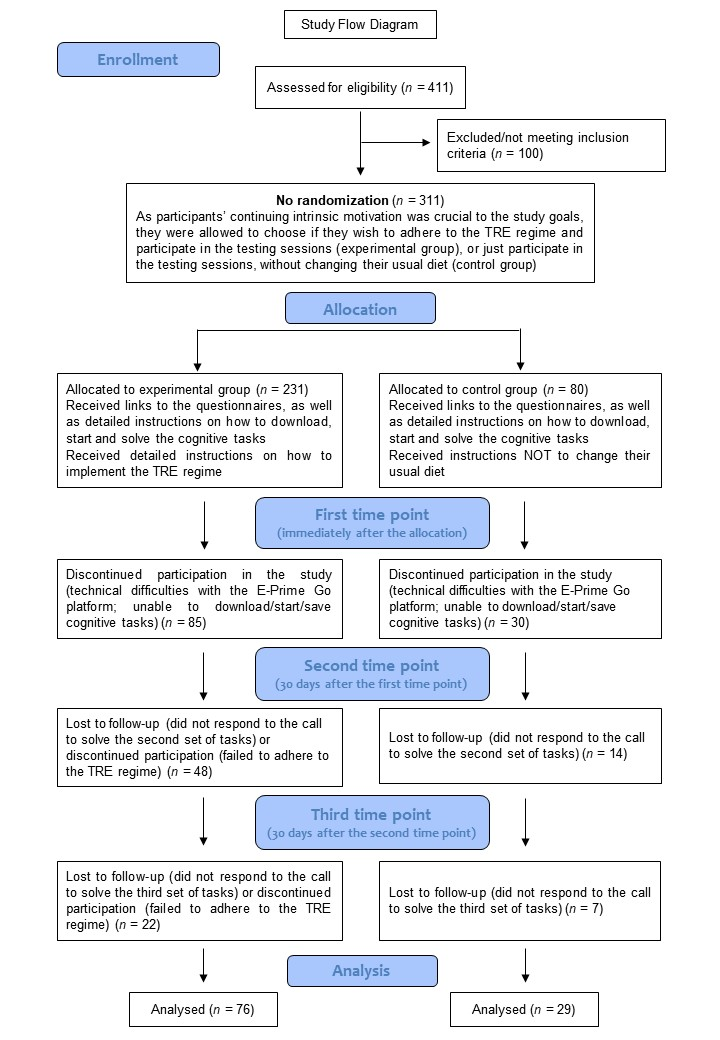
\includegraphics[scale=0.75]{media/image1.jpg}

    \caption{Study Flow Diagram}

    \label{fig:rId8}
  \end{fullwidth}


\end{figure*}








The gender composition of the participants who remained until the final time point in the study did not differ between groups (\emph{p~}<~.01, Fisher's exact test): There were 16 men and 60 women in the experimental group and seven men and 22 women in the control group. There were no significant differences between the control and experimental groups in age, height, and body mass index at the beginning of the study (see Table~1). Physical characteristics of the participants are shown in Table ~1.




\begin{table*}
  \begin{fullwidth}
    \caption{Physical characteristics of the participants}
    \begin{tabularx}{\linewidth}{@{} >{\RaggedRight\arraybackslash}m{9em} X X X X X X X X | X X X@{}}
      \toprule                                           & \multicolumn{4}{c}{Experimental group (\emph{n}=76)} &
      \multicolumn{4}{c}{Control group (\emph{n}=29)}    &                                                      &            &                                                                            \\

                                                         & \emph{M}                                             & \emph{SD}  & \emph{Min} & \emph{Max} & \emph{M} & \emph{SD}
                                                         & \emph{Min}                                           & \emph{Max} & \emph{t}   & \emph{p}   & \emph{d}                                         \\

      \hline Age                                         & 26.34                                                & 8.43       & 19         & 56         & 26.14    & 10.11     & 18   & 61  & 0.101 & .920
                                                         & 0.02                                                                                                                                           \\

      Height (cm)                                        & 172.22                                               & 8.93       & 150        & 196        & 170.50   & 8.38      & 155  & 186 & 0.884
                                                         & .379                                                 & 0.19                                                                                    \\

      Body mass index \newline (kg/m\textsuperscript{2}) & 24.06                                                & 2.97       & 19.27      & 33.79
                                                         & 22.60                                                & 2.68       & 18.78      & 30.39      & 0.022    & .982      & 0.50                      \\

      Lean body mass \newline (The Boer Formula)         & 51.20                                                & 6.67       & 36.51      & 73.39      & 48.93
                                                         & 5.88                                                 & 39.38      & 61.10      & 1.585      & .116     & 0.35                                  \\
      \bottomrule
    \end{tabularx}
  \end{fullwidth}
\end{table*}

\subsection{Instruments }



When applying for participation in the study via an online form, the participants reported their height and weight, from which their BMI was calculated. Four cognitive tests (objective measures of cognitive functioning) and two questionnaires (self-reported measures of sleeping quality and mood) were used at each testing session, as well as several follow-up questionnaires constructed ad hoc for the purposes of registering participants' adherence to the TRE regimen during the study. The questionnaires were administered via Google Forms, while the cognitive tasks were presented using E-Prime 3.0 software (Psychology Software Tools, Pittsburgh, PA).



\subsubsection{Attention}

The Attention Networking Test\textbf{ }(Fan et al., 2002; McConnell \& Shore, 2011) measures three aspects of attention: arousal (readiness to respond to a stimulus), directing attention (the selection of information from sensory input), and executive control (choosing between possible responses). After the initial instructions, the participants were shown arrows on the screen and their task was to decide the direction of the central arrow. If the arrows pointed to the left, they should have pressed the "1" button, if they pointed to the right, they should have pressed the "2" button. In the version used in this study arrows were presented in three uniform conditions that alternated by case: congruent (e.g. <\null<\null<\null<\null<), incongruent (e.g. >\null>\null<\null>\null>), or neutral (e.g. 00<00). During the trials, participants were presented with a fixation dot (1000 ms) in the center of the screen (no cue condition). In addition to the above, during some trials an asterisk was briefly displayed on the screen. If an asterisk was presented above or below the fixation point (spatial cue), arrows also appeared above or below. When the asterisk appeared in the center of the screen (central cue), arrows were presented either above or below the fixation point. All conditions were counterbalanced for each participant. Participants first went through a cycle of 12 trials after which they received performance feedback. The three aspects of attention are calculated as follows: The arousal score is obtained by subtracting the average reaction time in the central cue condition from the average reaction time in the no-cue condition. The attentional focus score is obtained by subtracting the average reaction time in the spatial cue condition from the average reaction time in the central cue condition. Finally, the executive control score is obtained by subtracting the average reaction time in the congruent condition from the average reaction time in the incongruent condition (McConnell \& Shore, 2011). In the present study, the test-retest correlations across three time points ranged between \emph{r} = .796 and \emph{r} = .878 for congruent conditions, between \emph{r} = .878 and \emph{r} = .906 for incongruent conditions, and between \emph{r} = .752 and \emph{r} = .859 for neutral conditions. Similarly, regarding conditions with different cues, the test-retest correlations ranged between \emph{r} = .801 and \emph{r }= .879 for conditions without cue, between \emph{r} = .824 and \emph{r }= .908 for spatial cue conditions, and between \emph{r} = .751 and \emph{r} = .879 for center cue conditions. As for scores extracted from the reaction times (RTs) across conditions, the test-retest correlations for the arousal and attention were low and ranged between \emph{r} = .247 and \emph{r} = .358 which is not unexpected, given the state and context dependent fluctuations in these functions. On the other hand, the executive control scores test-retest correlations ranged from \emph{r} =.691 to \emph{r} = 772.



\subsubsection{The memory span}
Two basic versions of memory tasks were used: Digit-Span Forward Task and Digit-Span Backward Task. In both versions, the participants are presented with a series of numbers, and their task is to repeat the presented numbers in the order in which they were presented (forwards) or in the reverse order of the presented ones (backwards; Bopp \& Verhaeghen, 2005). These two versions of the task provide somewhat different measures: The forward memory version primarily measures attention efficiency and short-term memory capacity, while the backward memory version measures the working memory capacity, as it requires participants to recruit the central executor (Giofrè et al., 2016; Kasper et al., 2012). Such a view is confirmed by the fact that the two versions correlate differently with measures of intelligence (Cornoldi et al., 2013) and that different neural circuits are activated when solving different versions (Rossi et al., 2013). In the computer version of the task, participants were presented with a series of digits on the screen, starting from a minimum of three to a maximum of nine digits. After the presentation of each sequence, the participant's task was to use the keyboard to type the presented sequence on the screen in the same order or in the reverse order, according to the type of task. For each sequence of digits, the respondent had two attempts, whereby, if the respondent answered correctly both times, the number of digits increased by one (up to nine digits), and if they answered incorrectly both times, the test stopped. The longest sequence of digits that the examinee accurately reproduces in each of the tasks represents the scope of their short-term and working memory. The test-retest correlations across three time points for the digit span forward ranged between\emph{ r} = .278 and \emph{r} = .371 -- again, these low correlations are not surprising, since attention is highly variable as a function of function of context and testing conditions, which could not be controlled in this study. For the digit span backward, the test-retest correlations ranged between \emph{r} = .430 and \emph{r} = .451.



\subsubsection{Working memory}
The Fixed N-Back task, which was used in this study, involves a continuous sequence of stimuli (pictorial or graphic) presented gradually. The participant's task is to determine whether the current stimulus is the same as the previous one or the one before it. To successfully solve the task, it is necessary to activate a number of cognitive processes: coding and temporary storage of a series of stimuli and continuous updating of upcoming stimuli. At the same time, irrelevant stimuli should be inhibited and removed from working memory, while current stimuli should be timely compared with those currently held in memory (Rac-Lubashevsky \& Kessler, 2016). The nature of the task requires the simultaneous recruitment of all the above-mentioned processes, which led to the classification of the N-back task among measures of working memory (Jaeggi et al., 2010). In our version of the task, the participants were shown letters on the screen, and they (considering the given rule) had to decide whether the presented letter was the target or not by clicking the “target” button. In the first condition, which served only to direct attention, only the letter Z was the target. In the 1-n back condition, a letter was the target if it was equal to the last letter that appeared before it. In the 2-n back condition, a letter was the target if it was equal to the penultimate letter presented. Considering the simplicity of the 1-n back condition, we decided to use only the average reaction time in the 2-n back condition as a measure of working memory. The test-retest correlations across three time points for the N-back score ranged between \emph{r} = .767 and \emph{r} = .842.



\subsubsection{Executive functions}
The classic Stroop task examines the inhibitory control, which is the participant's ability to inhibit automatic responses and select relevant sensory information (Miller \& Cohen, 2001). In the E-Prime 3.0. adaptation of the Stroop task, the participants were shown the names of colors (green, yellow, blue, red) on the screen, whereby the names were colored either in the same color as the written word (the word "yellow" colored in yellow) or in a different color (the word "yellow" colored blue), that is, the stimuli were congruent or incongruent. The participants' task was to determine in which color the word was written by pressing a predetermined key on the keyboard. Success in the task was determined as the average difference in reaction time to congruent and incongruent stimuli in milliseconds (ms), where a smaller difference indicates a greater inhibitory control. Participants first went through a cycle of eight trials, after which they received performance feedback. The test-retest correlations across three time points ranged between \emph{r} = .758 and \emph{r} = .838 for congruent conditions, and between \emph{r} = .815 and \emph{r} = .874 for incongruent conditions. The test-retest correlations for the Stroop score computed from these RTs ranged between \emph{r} = .589 and \emph{r} = .603.



\subsubsection{Sleep}

To measure sleep quality, the Pittsburgh Sleep Quality Index (PSQI; Buysse et al., 1989) was administered. This is a 19 items self-report questionnaire which aims to determine the participants' sleep quality on seven subscales: subjective sleep quality, sleep latency, sleep duration, habitual sleep efficiency, sleep disturbances, use of sleep medication, and daytime drowsiness. The scores range from 0 to 21 and the authors suggest that a score > 5 is to be considered a significant sleep disturbance. The reliability reported in earlier studies was between α =.70 and α =.83 (Mollayeva et al., 2016). In this study, McDonald's ω varied across time points between ω = .63 and ω = .68.


\subsubsection{Mood}

The Adjective Check List (ACL; Taub \& Berger 1974; Croatian translation and validation: Radošević-Vidaček et al., 1990), which consists of 57 adjectives that denote different emotional states, was used in this study. Participants had to respond to what extent they experienced certain emotions that day, on a scale ranging from 0 (“Not at all”) to 4 (“Extremely”). Average scores were computed for eight dimensions: anxiety (six items), depression (six items), fatigue (eight items), hostility (eight items), friendliness (five items), cheerfulness (five items), concentration (eight items), and energy (six items). The internal reliability coefficients of the subscales were high, ranging from ω = .78 for concentration to ω = .92 for fatigue.



\subsection{Procedure }



The study was conducted over a period of 2 months (May-July 2021) online, via the Google Forms for the questionnaires and E-PrimeGo (version 3.0) platform for the cognitive tests. After filling in the initial questionnaire, the participants received an e-mail confirming or rejecting their participation in the study with a detailed explanation. All participants received instructions for solving the tasks and filling in the questionnaires prior to the first testing session. Participants could access the E-PrimeGo test base using a link provided by the researcher. Their answers were automatically saved in an online database accessible only to the researchers. Video instructions on the installation of the tasks were sent to the participants, as well as instructions for solving potential technical difficulties. The participants were given 3 days to solve all the tests of the first session. They were instructed to start the session only if they were able to do so in a quiet environment without any distractions.



After the completion of the first testing session, participants in the experimental group received detailed instructions for starting TRE. They were introduced to the concept of TRE, and its benefits and risks. Along came the instruction that in the next two months they should adhere to the TRE, for which they alternate between a 16-hour fasting window and an 8-hour eating window. Participants were given the choice to decide when to start their fasting/eating window, with the instruction that they maintain a routine (e.g. if they decide to start their fasting window at 5pm, it is important that they maintain that routine every day). The participants were encouraged to not drastically change the type of food they consume and to pay attention to the intake of enough nutrients in the eating window. During the fasting window, participants were allowed to consume water, unsweetened tea and coffee. In the first week, participants were allowed to maintain a fasting window of 14 hours and an eating window of 10 hours to facilitate the participants' transition to a full fast of 16 hours. Also, we encouraged the subjects to take one day a week "off" from fasting, during which they would not pay attention to the time intervals of eating and fasting. Participants from the control group were instructed not to adhere to any new diet during the participation in the study, but they were included in all the same consecutive testing sessions as the participants from the experimental group.


\begin{figure}
  \begin{fullwidth}
    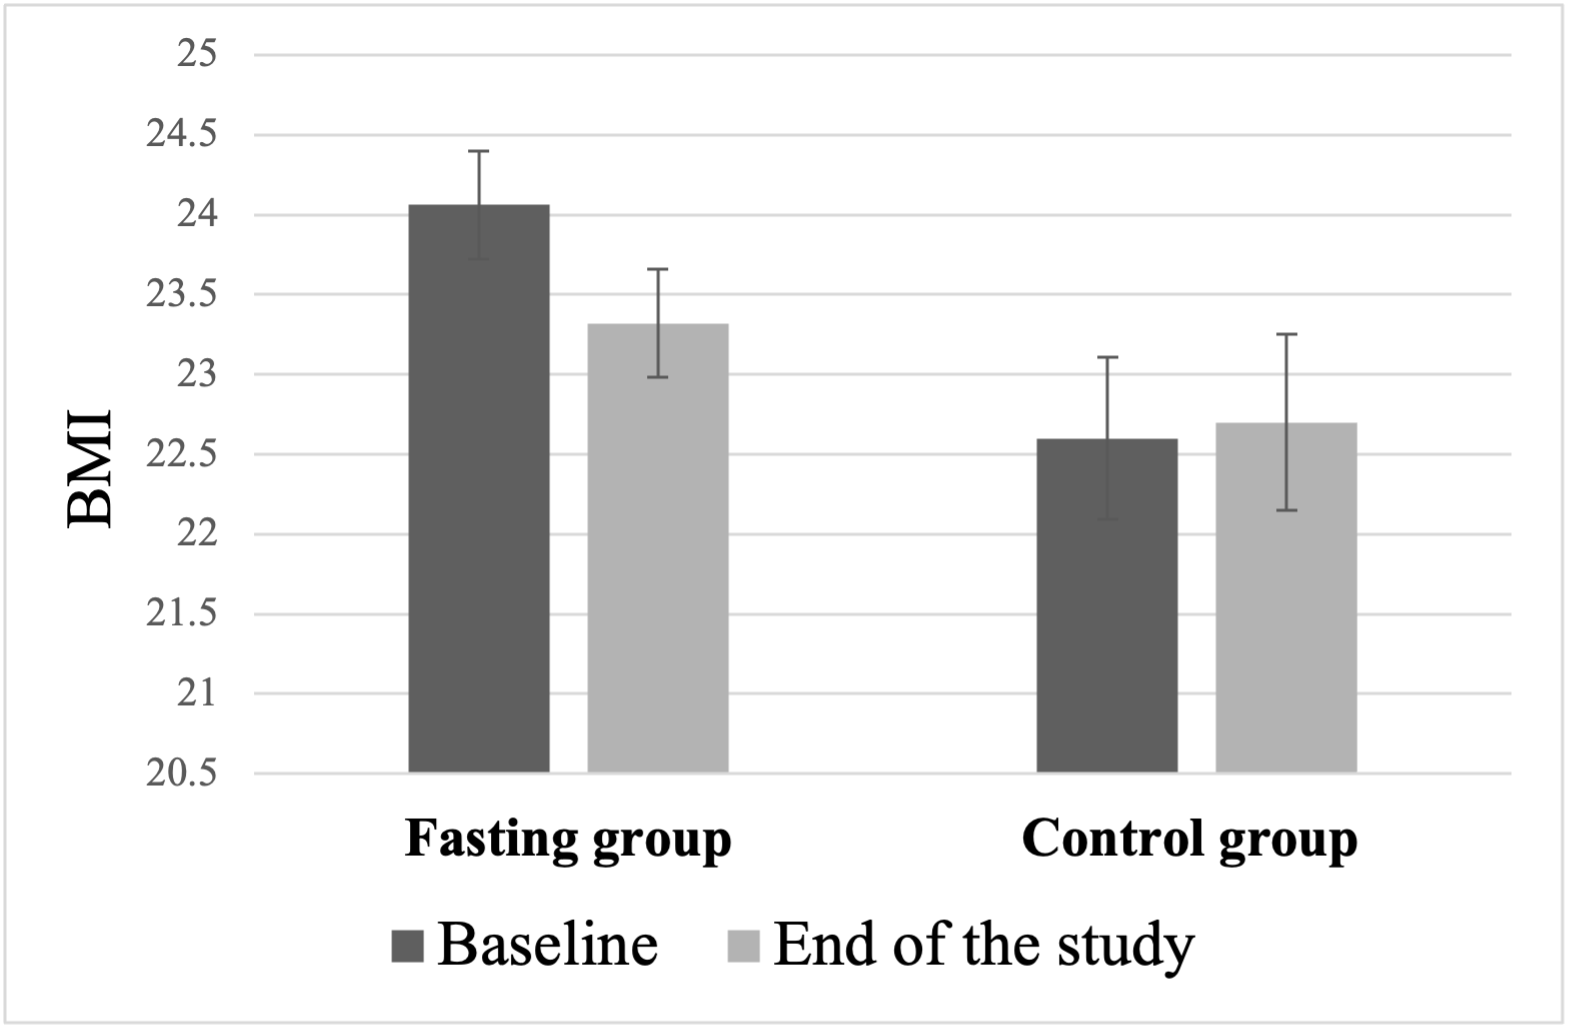
\includegraphics[width=\linewidth]{media/image2.png}
    \caption{BMI at the baseline and at the end of the study (following two months of intermittent fasting regime for the experimental group and no dietary changes in the control group). Error bars represent standard errors.}

  \end{fullwidth}
\end{figure}


The second testing session took place 1 month after the first session, and the third session took place 2 months after the first one. Due to an online participation and different work/life schedules of participants, there was no fixed time of day when participants were instructed to do the testing. The testing announcements were sent out in the morning exactly a month (and two months) after the first testing took part, and there was an instruction to finish all the tests and fill out the questionnaires in 3 days. Participants completed all cognitive tests and filled the mood and sleep questionnaires, as well as control questionnaires about weight loss and the adherence to the TRE protocol.



Throughout the study, we maintained regular contact with the participants in order to motivate them to stay in the dietary regimen and keep completing the cognitive tests, and to address any of their doubts and questions. Participants from the experimental group could join a private group on Facebook, in which tips for more efficient adherence to fasting and answers to the most common questions were published, and the participants themselves could comment and start discussions. All contents published in the group have been reviewed and approved by a MSc nutritionist, who also held an online lecture for the participants in order to familiarize them with intermittent fasting in more detail. A summary and the most important tips were sent to the e-mail addresses of all participants who could not participate in the online lecture.


\subsection{Statistical analyses}
% \vspace*{1px}

For each dependent variable, we conducted an analysis of variance for repeated measures with the group (experimental vs. control) as a source of variance between participants and time-point (1\textsuperscript{st}/2\textsuperscript{nd}/3\textsuperscript{rd}) as a within-group source of variance. In instances where Mauchly's test of sphericity showed that variances between groups differed, Greenhouse-Giesser correction was applied.


\section{Results }



\subsection{Weight loss}



Although weight loss was not a primary focus of this study, we considered the changes in BMI as objective indicators of successful adherence to the intermittent fasting regimen. The repeated measures ANOVA showed a significant time x group interaction, \emph{F}(1, 102) = 31.32, \emph{p} < .001, η\textsubscript{p}\textsuperscript{2} = .235. As can be seen in Figure 2, the interaction stemmed from the fact that the average BMI in the experimental group was lower at the end of the study compared to the baseline, \emph{t}(75) = 8.86; \emph{p < }.001; \emph{d} = 0.25, while the average BMI in the control group did not change significantly, \emph{t}(27) = -1.11; \emph{p }= .27; \emph{d} = 0.03.








\subsection{Performance on cognitive tests}



As can be seen in Table 2, there was a significant increase in scores on the executive control segment of the Attention Networking Test, digit span forward, N-back, and Stroop as a function of time point. However, there were no significant differences between the experimental and the control group, and no significant group x time-point interactions, which implies that these improvements were a result of practice and familiarity with the task, and not the TRE regimen per se.



















































\begin{table*}[t]
  \begin{fullwidth}
    \caption{Scores on cognitive tasks (attention, memory, executive functions) across time points for experimental and control group, and the results of repeated measures ANOVAs, with group (experimental vs. control) as a source of variance between participants and time point (1\textsuperscript{st}/2\textsuperscript{nd}/3\textsuperscript{rd}) as a within-group source of variance.}

    \resizebox{\textwidth}{!}{%
      \begin{tabular}{@{} l l l l l l l | l l l l l @{}}
        \toprule                                       & \multicolumn{2}{c}{\textbf{First time point}} &
        \multicolumn{2}{c}{\textbf{Second time point}} &
        \multicolumn{2}{c}{\textbf{Third time point}}  &                                               &                      &                      &               &                                                                                              \\

                                                       & \multicolumn{2}{l}{}                          & \multicolumn{2}{l}{} & \multicolumn{2}{l}{} &               &                                       &         &

                                                       &                                                                                                                                                                                                            \\

                                                       & \textbf{Expmtl.}                              & \textbf{Control }    & \textbf{Expmtl.}     &
        \textbf{Control }                              & \textbf{Expmtl.}                              & \textbf{Control }    &                      &               &                                       &
                                                       &                                                                                                                                                                                                            \\


        \hline                                         & \emph{M (SD)}                                 & \emph{M (SD)}        & \emph{M (SD)}        & \emph{M (SD)} & \emph{M (SD)}
                                                       & \emph{M (SD)}                                 &                      & \emph{F}             & \emph{p}      & η\textsubscript{p}\textsuperscript{2}
        \\

        \textbf{Attention}                             &                                               &                      &                      &               &                                       &         &                    &       &      &      & \\

        \hline Arousal                                 & 14.70                                         & 14.61                & 14.84                & 15.11
                                                       & 9.62                                          & 13.48                & Time point           &
        0.39                                           & .67                                           & .004                                                                                                                                                       \\
                                                       & (32.05)                                       & (20.65)              & (21.29)              & (23.69)       & (26.25)                               & (21.26) & Group              & 0.18  & .65  & .002 & \\
                                                       &                                               &                      &                      &               &                                       &         & Time point x group & 0.13  & .88  & .001
        \\

        \hline Directing attention                     & 23.05                                         & 12.04                & 23.39                & 14.70         & 22.67                                 & 14.95   & Time point         & 0.07  & .93  & .001   \\
                                                       & (31.98)                                       & (26.64)              & (32.02)              & (25.75)       & (28.12)                               & (24.13) & Group              & 4.08  & .05  & .041   \\
                                                       &                                               &                      &                      &               &                                       &         & Time point x group & 0.08  & .93  & .001   \\

        \hline Executive control                       & 129.16                                        & 128.38               & 106.08               & 99.10         & 94.36                                 & 83.55   & Time point         & 21.92 & .001 & .187   \\
                                                       & (87.35)                                       & (60.92)              & (76.82)              & (37.33)       & (48.42)                               & (27.25) & Group              & 0.21  & .65  & .002   \\
                                                       &                                               &                      &                      &               &                                       &         & Time point x group & 0.34  & .71  & .004   \\

        \hline \textbf{Memory}                         &                                               &                      &                      &               &                                       &         &                    &       &      &      & \\

        \hline Digit span forward                      & 7.24                                          & 6.81                 & 7.45                 & 7.30          & 7.48                                  & 7.41    & Time point         & 5.15  & .007 & .051   \\
                                                       & (0.96)                                        & (1.08)               & (1.03)               & (1.07)        & (1.04)                                & (1.05)  & Group              & 1.68  & .42  & .017   \\
                                                       &                                               &                      &                      &               &                                       &         & Time point x group & 0.88  & .20  & .009   \\

        \hline Digit span backward                     & 6.13                                          & 6.08                 & 6.37                 & 6.32          & 6.56                                  & 6.40    & Time point         & 2.24  & .11  & .024   \\
                                                       & (1.40)                                        & (1.04)               & (1.38)               & (1.28)        & (1.23)                                & (1.04)  & Group              & 0.16  & .69  & .002   \\
                                                       &                                               &                      &                      &               &                                       &         & Time point x group & 0.06  & .94  & .001   \\

        \hline N-back                                  & 1.75                                          & 1.81                 & 1.95                 & 1.64          & 2.04                                  & 2.20    & Time point         & 9.07  & .001 & .092   \\
                                                       & (0.93)                                        & (0.83)               & (0.82)               & (0.89)        & (0.96)                                & (0.97)  & Group              & 0.33  & .57  & .004   \\
                                                       &                                               &                      &                      &               &                                       &         & Time point x group & 0.70  & .49  & .008   \\

        \textbf{Executive functions}                   &                                               &                      &                      &               &                                       &         &                    &       &      &      & \\

        \hline Stroop test                             & 168.78                                        & 192.05               & 124.28               & 114.17        & 80.12                                 & 68.89   & Time point         & 32.11 & .001 & .251   \\
                                                       & (151.71)                                      & (124.63)             & (133.13)             & (78.73)       & (82.12)                               & (68.34) & Group              & 0.01  & .98  & .000   \\
                                                       &                                               &                      &                      &               &                                       &         & Time point x group & 1.09  & .34  & .011   \\
        \bottomrule
      \end{tabular}}
  \end{fullwidth}
\end{table*}




\subsection{Self-report measures}



As can be deduced from Table 3, there were several significant differences in mood dimensions as a function of the time point: Participants scored lower on anxiety, depression, and fatigue, and higher on cheerfulness and energy at the end of the study, compared to the pre-intervention testing. However, as in the case of cognitive tests, there were no differences between groups, and no group x time point interactions, implying that these shifts in mood cannot be ascribed to the TRE regimen either.








\begin{table*}[th!]
  \begin{fullwidth}
    \caption{Scores on mood and sleep quality questionnaires across time points for experimental and control group, and the results of mixed model repeated measures ANOVAs, with group (experimental vs. control) as a source of variance between participants and time point (1\textsuperscript{st}/2\textsuperscript{nd}/3\textsuperscript{rd}) as a within-group source of variance.
    }
    \resizebox{\textwidth}{!}{%
      \begin{tabular}{@{} l l l l l l l | l l l l l @{}}

        \toprule                                       & \multicolumn{2}{c}{\textbf{First time point}} &
        \multicolumn{2}{c}{\textbf{Second time point}} &
        \multicolumn{2}{c}{\textbf{Third time point}}  &                                               &                      &                      &               &                                                                                          \\

                                                       & \multicolumn{2}{l}{}                          & \multicolumn{2}{l}{} & \multicolumn{2}{l}{} &               &                                       &        &

                                                       &                                                                                                                                                                                                        \\

                                                       & \textbf{Expmtl.}                              & \textbf{Control }    & \textbf{Expmtl.}     &
        \textbf{Control }                              & \textbf{Expmtl.}                              & \textbf{Control }    &                      &               &                                       &
                                                       &                                                                                                                                                                                                        \\


        \hline                                         & \emph{M (SD)}                                 & \emph{M (SD)}        & \emph{M (SD)}        & \emph{M (SD)} & \emph{M (SD)}
                                                       & \emph{M (SD)}                                 &                      & \emph{F}             & \emph{p}      & η\textsubscript{p}\textsuperscript{2}
        \\

        \hline   Anxiety                               & 0.84                                          & 0.87                 & 0.95                 & 0.99          & 0.63                                  & 0.71   & Time point         & 4.66 & .01  & .045 \\
                                                       & (0.80)                                        & (0.77)               & (0.96)               & (0.85)        & (0.78)                                & (0.62) & Group              & 0.17 & .68  & .002 \\
                                                       &                                               &                      &                      &               &                                       &        & Time point x group & 0.01 & .99  & .000 \\

        \hline Depression                              & 0.86                                          & 0.95                 & 0.84                 & 0.90          & 0.62                                  & 0.65   & Time point         & 4.72 & .01  & .045 \\
                                                       & (0.81)                                        & (0.75)               & (0.86)               & (0.67)        & (0.76)                                & (0.63) & Group              & 0.37 & .54  & .004 \\
                                                       &                                               &                      &                      &               &                                       &        & Time point x group & 0.07 & .94  & .001 \\

        \hline Fatigue                                 & 1.42                                          & 1.64                 & 1.30                 & 1.87          & 1.24                                  & 1.35   & Time point         & 3.21 & .04  & .031 \\
                                                       & (0.98)                                        & (0.97)               & (0.98)               & (1.03)        & (0.96)                                & (1.09) & Group              & 2.74 & .10  & .027 \\
                                                       &                                               &                      &                      &               &                                       &        & Time point x group & 1.86 & .16  & .018 \\

        \hline Hostility                               & 0.47                                          & 0.50                 & 0.45                 & 0.52          & 0.38                                  & 0.37   & Time point         & 2.03 & .13  & .020 \\
                                                       & (0.54)                                        & (0.67)               & (0.68)               & (0.69)        & (0.57)                                & (0.49) & Group              & 0.09 & .76  & .001 \\
                                                       &                                               &                      &                      &               &                                       &        & Time point x group & 0.42 & .65  & .004 \\

        \hline Friendliness                            & 2.44                                          & 2.53                 & 2.55                 & 2.45          & 2.64                                  & 2.73   & Time point         & 2.34 & .09  & .023 \\
                                                       & (0.97)                                        & (0.91)               & (0.91)               & (0.98)        & (0.96)                                & (0.98) & Group              & 0.01 & .95  & .000 \\
                                                       &                                               &                      &                      &               &                                       &        & Time point x group & 0.46 & .64  & .005 \\

        \hline Cheerfulness                            & 2.11                                          & 2.24                 & 2.26                 & 2.14          & 2.43                                  & 2.54   & Time point         & 5.03 & .007 & .048 \\
                                                       & (1.00)                                        & (0.66)               & (0.95)               & (0.82)        & (0.92)                                & (0.96) & Group              & 0.01 & .98  & .000 \\
                                                       &                                               &                      &                      &               &                                       &        & Time point x group & 0.69 & .50  & .007 \\

        \hline Concentration                           & 2.40                                          & 2.48                 & 2.58                 & 2.35          & 2.63                                  & 2.56   & Time point         & 1.36 & .26  & .014 \\
                                                       & (0.76)                                        & (0.70)               & (0.75)               & (0.62)        & (0.78)                                & (0.84) & Group              & 0.38 & .54  & .004 \\
                                                       &                                               &                      &                      &               &                                       &        & Time point x group & 1.12 & .33  & .011 \\

        \hline Energy                                  & 1.75                                          & 1.81                 & 1.95                 & 1.64          & 2.04                                  & 2.20   & Time point         & 6.04 & .003 & .058 \\
                                                       & (0.93)                                        & (0.83)               & (0.82)               & (0.89)        & (0.96)                                & (0.97) & Group              & 0.05 & .82  & .001 \\
                                                       &                                               &                      &                      &               &                                       &        & Time point x group & 2.16 & .14  & .021 \\


        \hline        Sleep quality (PSQI)             & 5.21                                          & 4.44                 & 4.00                 & 4.67          & 4.72                                  & 4.72   & Time point         & 0.76 & .47  & .015 \\
                                                       & (3.23)                                        & (1.95)               & (2.61)               & (2.76)        & (2.76)                                & (2.76) & Group              & 0.02 & .89  & .000 \\
                                                       &                                               &                      &                      &               &                                       &        & Time point x group & 0.89 & .14  & .040 \\
        \bottomrule
      \end{tabular}}
  \end{fullwidth}
\end{table*}





\section{Discussion }



The aim of this study was to determine how TRE affects cognitive functions and mental health, that is, whether fasting for 16 hours a day throughout two months would lead to significant improvements in attention, memory, executive skills, mood, and sleep quality.



\subsection{The impact of TRE on cognitive functions.}



We found no effect of TRE on cognitive performance. Scores on several cognitive tasks improved significantly across time points, but for both groups. Given that there were no significant group x time point interactions, it is most likely that the observed trend was caused by familiarity with the tasks and solving strategies (Wesnes \& Pincock, 2002). Previous studies reported mixed findings, with some reporting positive effects of intermittent fasting on cognitive measures (Giles et al., 2012; Colzato et al., 2013; Farooq et al., 2010; 2015; Teong et al., 2021), while others found no effect (Ghayour Najafabadi et al., 2015; Harder et al., 2017; Rachid et al., 2021), or even negative effects, at least in the case of short-term fasting (Benau et al., 2014; 2021). There might be numerous methodological reasons we failed to observe significant change in cognitive functioning of the fasting group (see limitations section for more details), and the lack of evidence does not prove that an effect does not exist. Nonetheless, it is still worth noting that across seven measures in three domains of cognitive functioning, none showed a significant group x time interaction. Thus, there is a possibility that the positive effects of intermittent fasting on domains beyond weight loss are overemphasized in the media and popularized without adequate evidence (Johnstone, 2014). Caution might prove especially important in cases where there is a risk that fasting could be a sort of gateway to extreme food restrictions and other harmful behaviors. It has already been shown that intermittent fasting is related to eating disorder behaviors and psychopathology (Ganson et al., 2022).



The most researched dietary intervention in humans is still caloric restriction, and conclusions are then generalized to similar dietary regimens such as intermittent fasting. Although caloric restriction and intermittent fasting have similar effects (Teong et al., 2021), it should be emphasized that intermittent fasting does not necessarily limit the amount of food consumed. Some studies showed that fat tissue loss can occur even without caloric restriction (Moro et al., 2016). Furthermore, it seems that the type of consumed food also has an impact on cognitive functions. Thus, for example, a diet with a high fat content is associated with worse performance in cognitive tasks (Edwards et al., 2011). In a recent systematic review, it has been concluded that the observed cognitive benefits were associated more with other interventions, such as decreasing the caloric intake without a complete fasting period, weight loss, dietary approaches to stop hypertension, blood pressure reduction, and exercise, rather than with intermittent fasting per se (Senderovich et al., 2023).



One possible explanation for the lack of effect found in this study, is the low level of control the researchers had over the type and amount of food consumed, and the partcipants' weight measurement. Since in our study we did not control the type and amount of food consumed, and the participants measured their own weight, greater control over the aforementioned factors is recommended in future studies. Another possible explanation for the lack of effect is that the adherence to the diet in our sample was not strict enough. Participants who did not fast for at least 14 hours a day throughout the duration of the study (based on their self-reported adherence) were excluded from the final analyses, but a greater control of time periods and the number of days spent fasting is needed. That being said, we have reason to believe that our participants were highly intrinsically motivated and that they did adhere to the time restricted eating regime to the best of their possibilities: 71\% of participants from the experimental group reported that they planned to continue with the intermittent fasting even after the completion of the study. This is in line with the claims that this particular dietary regime is easy to implement and adhere to, even in the long run. In fact, it might be argued that its implementation becomes even easier as a function of time, as it has previously been shown that contrary to the effects of short-term, selective food deprivation, long-term energy restriction decreases food cravings (Meule, 2020).



\subsection{Impact of intermittent fasting on mood and sleep quality.}



We also examined whether the participants' mood and sleep quality changed in the context of intermittent fasting. Again, the only significant effects were related to the time point: Participants scored lower on anxiety, depression, and fatigue, and higher on cheerfulness and energy at the end of the study, compared to the pre-intervention testing. However, there were no differences between groups, or group x time point interactions in either of the mood dimensions, or in sleep quality. Given that the research was conducted in the period from May to July, the positive changes in the mood of both groups could be linked to the arrival of Summer months and the positive effects of sunny weather on mood (Keller et al., 2005). Summer vacations might have also influenced this increase in positive and decrease in negative moods.



Our findings are in line with some previous studies, showing that that neither a short-term two-day fast nor an intermittent fast lasting 8 weeks has any effect on the mood of the participants or on the quality of sleep (Solianik \& Sujeta, 2018; Teong et al., 2021). The assumptions about the positive influence of fasting on mood are based primarily on studies of the clinical population, where dietary interventions have shown significant potential in improving the symptoms of mood disorders in obese participants with frequent comorbidities (Patsalos et al., 2021). Although some studies showed that intermittent fasting might have potential for improving mood (Bowen et al., 2018) and reducing depressive symptoms (Hussin et al., 2013) in non-clinical populations, it is possible that the same dietary interventions have greater implications for clinical populations. Additionally, gender differences were found in the impact of fasting on the reduction of anxiety (with a significant reduction being observed in men only; Nugraha et al., 2020) and due to the small number of male participants, we could not address this question in this study. Finally, different measures of mood and different fasting regimens were used in various studies, so due to the lack of uniform designs using TRE, only limited conclusions can be drawn.

\begin{originalPurpose}

  Intermittent fasting drew attention among scientists in fields outside of nutrition, due to reports of its positive effects on psychological well-being. However, in most studies that link dietary regimens to cognitive functions, some form of caloric restriction was used as a dietary intervention. Given the lack of research linking intermittent fasting and a person's psychological health and cognitive functioning, the goal of this study was to contribute to the literature investigating the potential benefits of intermittent fasting, with a more comprehensive approach. This included a battery of cognitive tests (objective measures of cognitive functioning) as well as reports of mood (subjective measures of psychological functioning) and sleep quality, as it has been suggested that intermittent fasting regulates circadian rhythms and thus affects psychological outcomes.

\end{originalPurpose}


Recently, it has been suggested that intermittent fasting has a positive effect on sleep through the regulation of circadian rhythms (Chaix et al., 2019). We were not able to show any significant effect of fasting on sleep quality, although the results did show a certain amount of improvement in PSQI score (at baseline, fasting group had the average score slightly above 5, which is clinically indicative for impaired sleep quality, dropping below 5 by the second time point). In future, larger studies, it would be interesting to check whether quality of sleep has a mediating influence on the relationship between intermittent fasting and performance on cognitive tasks, considering that there is no research that connects the mentioned variables into one complete model.








\subsection{Limitations of the current study and recommendations for future research}



The major limitation of this study was the lack of randomization. As previously described, due to the nature of the research topic, and the fact that the participants did not receive any financial incentives, their intrinsic motivation was the only factor ensuring their continuing cooperation (both in adhering to the TRE, and in participating in testing sessions). Thus, their preferences were accommodated, at the cost of internal validity of the study. Similarly, there was no control over the exact time of day when the participants started fasting, which might be crucial, as it has been speculated that intermittent fasting has an impact on circadian rhythms. The participants in this study were instructed to start the fasting period in the evening, because interventions with reduced food intake in the evening have been shown to be more effective (Jakubowicz et al., 2013), but due to differences in the schedule and working hours of the participants, they were allowed to decide for themselves when to start with the fasting period. Eating food late in the evening can disrupt circadian rhythms and consequently performance in cognitive tests (Currenti et al., 2021). Future studies should equalize fasting conditions for all subjects, and/or consider the interindividual differences in morningness - eveningness in order to determine whether there are differences in time-restricted day versus night interventions. Related to this, another potentially important element we could not control for was the time of day when participants took the tests and filled the questionnaires -- both circadian rhythms and timing in relation to fasting window could have influenced the performance on tests. As we argued above, we opted to achieve higher ecological validity, aiming to assess the outcomes of the type of time restricted eating regime people actually implement in real life, not laboratory conditions, though this comes at a cost of internal validity.





Additionally, online testing - as opposed to testing in a lab setting - could have impaired the validity of the results. Solving the tests without the presence of the researcher could have led to uneven conditions among the participants, starting from physical surroundings, the presence of other people in the room, to interrupting the testing and solving the tests at different intervals.


Last, but not least, our control group was disproportionately smaller than the fasting group, and by the end of the study, fewer than 30 participants remained in it. This was an oversight on our part: We had expected a large dropout in the experimental group (because adherence to any fasting regime is challenging) and minimal dropout in the control group (because they only had to solve the tasks and fill the questionnaires on three occasions -- all online, no dietary or any other lifestyle changes were required). Ultimately, however, the dropout in both groups was large. We are very grateful to one of the reviewers of this paper (Dr. Sean Devine) who pointed out that imbalanced sample sizes between groups decrease power in repeated-measures designs. He also took the time to conduct a simulation-based power analysis using multilevel modeling to account for the uneven sample sizes. Depending on the expected effect size he used, he found that the current dataset would only have power to detect a small interaction effect size (β = .1 or β = .2) 17\% to 50\% of the time, respectively. This implies that the study was very likely underpowered to detect the effects of these magnitudes. While we agree whole-heartedly with the fact that this sample size would not enable us to detect such small effects, we also have to draw the readers' attention to the main point of this manuscript, which is calling for the caution in advising dietary restrictions and taking into account costs and benefits of such restrictions. We used the smallest possible effects size in our calculations of the statistical power: Even if the effect was detected, future studies might try to assess the applicability of such small effects in real-life, especially when therapeutic benefits are expected, and even more so when the interventions are not without potential adverse effects.


\section{Conclusion }



Questions ranging from seemingly simple ones, such as what best defines dieting or restrained eating to the methodologically complex ones, such as which approaches to the assessment of eating behaviors are optimal, are often a matter of debate even among the experts (for a detailed review see Meule, 2023). To laymen, especially those in search of solutions for their physical or mental health related problems, setting realistic expectations and even more so assessing the effectiveness of a dietary intervention on themselves beyond the objective measure of weight loss is necessarily distorted by the various processes of motivated reasoning. Using a set of objective cognitive tasks, we found no substantial effect of the intermittent fasting on either the tested cognitive functions (attention, memory, working memory, executive functions), throughout the time period of two months. Similarly, we found no substantial effect of fasting on any of the dimensions of mood (anxiety, depression, fatigue, hostility, friendliness, cheerfulness, concentration, energy) or on sleep quality. Although the mechanisms underlying the impact of fasting on cognitive functions have been described in detail and show potential in animal models (Dias et al., 2021), research on humans is very limited.



Variational research designs represent an additional problem in drawing conclusions. Researchers have used different fasting regimens, where very often all regimens are classified under a common denominator, although the fasting period takes place at different times and are of different durations. Ramadan fasting, of which effects on cognition are most often observed, takes place during the day, so it is not directly comparable to other fasting regimens in which the fasting period takes place at night. With the given body of evidence, it seems that when it comes to recommending fasting dietary regimens, greater care should be put into avoiding exaggerated claims about the benefits which transcend those related to physical health, primarily regulation of weight.





\section{Funding}



The license for the E-Prime Go v3 was funded by the internal grant no. 11-929-1027 (Faculty of Humanities and Social Sciences). No other segments of the study were funded.



\section{Acknowledgments}



The authors would like to thank Anja Bašnec, a M.Sc. nutritionist, affiliated with Food technology faculty in Osijek, J.J.S. University, Croatia, for her generous help with preparing the educational materials for the participants in the experimental group.






\section{References }



% \hspace*{\parindent}Anton, S. D., Moehl, K., Donahoo, W. T., Marosi, K., Lee, S. A., Mainous, A. G., Leeuwenburgh, C., \&, Mattson, M. P. (2017). Flipping the metabolic switch: Understanding and applying the health benefits of fasting.\emph{ Obesity, 26}(2), 254--268. \url{https://doi.org/10.1002/oby.22065}



% Antoni, R., Johnston, K. L., Collins, A. L., \& Robertson, M. D. (2017). Effects of intermittent fasting on glucose and lipid metabolism. \emph{Proceedings of the Nutrition Society}, \emph{76}(3), 361-368. \url{https://doi.org/10.1017/s0029665116002986}



Appleton, K. M., \& Baker, S. (2015). Distraction, not hunger, is associated with lower mood and lower perceived work performance on fast compared to non-fast days during intermittent fasting.\emph{ Journal of Health Psychology, 20}(6), 702--711. \url{https://doi.org/10.1177/1359105315573430}



Arnold, S. E., Arvanitakis, Z., Macauley-Rambach, S. L., Koenig, A. M., Wang, H.-Y., Ahima, R. S., Craft, S., Gandy, S., Buettner, C., Stoeckel, L. E., Holtzman, D. M., \& Nathan, D. M. (2018). Brain insulin resistance in type 2 diabetes and Alzheimer disease: Concepts and conundrums.\emph{ Nature Reviews Neurology, 14}(3), 168--181\emph{.} \url{https://doi.org/10.1038/nrneurol.2017.185}



% Arnoldussen, I. A., Kiliaan, A. J., \& Gustafson, D. R. (2014). Obesity and dementia: Adipokines interact with the brain. \emph{European Neuropsychopharmacology}, \emph{24}(12), 1982-1999. \url{https://doi.org/10.1016/j.euroneuro.2014.03.002}



% Axelrod, D. A., \& Hayward, R. (2007). Nonrandomized interventional study designs (quasi-experimental designs). In: D. F. Penson \& J. T. Wei (Eds.), \emph{Clinical Research Methods for Surgeons} (pp.63-76). Humana Totowa. \url{https://doi.org/10.1007/978-1-59745-230-4}



% Backhaus, J., Junghanns, K., Broocks, A., Riemann, D., \& Hohagen, F. (2002). Test--retest reliability and validity of the Pittsburgh Sleep Quality Index in primary insomnia. \emph{Journal of Psychosomatic Research}, \emph{53}(3), 737-740. \url{https://doi.org/10.1016/s0022-3999(02)00330-6}



% Barnosky, A. R., Hoddy, K. K., Unterman, T. G., \& Varady, K. A. (2014). Intermittent fasting vs daily calorie restriction for type 2 diabetes prevention: a review of human findings. \emph{Translational Research}, \emph{164}(4), 302-311. \url{https://doi.org/10.1016/j.trsl.2014.05.013}



% Bear, T., Dalziel, J., Coad, J., Roy, N., Butts, C., \& Gopal, P. (2021). The microbiome-gut-brain axis and resilience to developing anxiety or depression under stress. \emph{Microorganisms}, \emph{9}(4), Article 723. \url{https://doi.org/10.3390/microorganisms9040723}



Bedrosian, T. A., \& Nelson, R. J. (2017). Timing of light exposure affects mood and brain circuits. \emph{Translational Psychiatry}, \emph{7}(1), e1017-e1017. \url{https://doi.org/10.1038/tp.2016.262}



% Bekinschtein, P., Cammarota, M., \& Medina, J. H. (2014). BDNF and memory processing. \emph{Neuropharmacology}, \emph{76}, 677-683. \url{https://doi.org/10.1016/j.neuropharm.2013.04.024}



Benau, E. M., Makara, A., Orloff, N. C., Benner, E., Serpell, L., \& Timko, C. A. (2021). How does fasting affect cognition? An updated systematic review (2013-2020). \emph{Current Nutrition Reports}, \emph{10}(4), 376--390. \href{https://doi.org/10.1007/s13668-021-00370-4}{https://doi.org/10.1007/s13668-021-00370-4}



Benau, E. M., Orloff, N. C., Janke, E. A., Serpell, L., \& Timko, C. A. (2014). A systematic review of the effects of experimental fasting on cognition. \emph{Appetite}, \emph{77}, 52--61. \href{https://doi.org/10.1016/j.appet.2014.02.014}{https://doi.org/10.1016/j.appet.2014.02.014}



% Boer, P. (1984). Estimated lean body mass as an index for normalization of body fluid volumes in man. \emph{American Journal of Physiology}, \emph{247}(4 pt 2), F632-F635. \url{https://doi.org/10.1152/ajprenal.1984.247.4.F632}



Bopp, K. L., \& Verhaeghen, P. (2005). Aging and verbal memory span: A meta-analysis. \emph{The Journals of Gerontology Series B: Psychological Sciences and Social Sciences}, \emph{60}(5), P223-P233. \url{https://doi.org/10.1093/geronb/60.5.p223}



Bowen, J., Brindal, E., James-Martin, G., \& Noakes, M. (2018). Randomized trial of a high protein, partial meal replacement program with or without alternate day fasting: Similar effects on weight loss, retention status, nutritional, metabolic, and behavioral outcomes. \emph{Nutrients}, \emph{10}(9), Article 1145. \url{https://doi.org/10.3390/nu10091145}



% Burke, T. M., Scheer, F. A., Ronda, J. M., Czeisler, C. A., \& Wright Jr, K. P. (2015). Sleep inertia, sleep homeostatic and circadian influences on higher-order cognitive functions. \emph{Journal of Sleep Research}, \emph{24}(4), 364-371. \url{https://doi.org/10.1111/jsr.12291}



Buysse, D. J., Reynolds III, C. F., Monk, T. H., Berman, S. R., \& Kupfer, D. J. (1989). The Pittsburgh Sleep Quality Index: A new instrument for psychiatric practice and research. \emph{Psychiatry Research}, \emph{28}(2), 193-213. \url{https://doi.org/10.1016/0165-1781(89)90047-4}



Ceppa, F., Mancini, A., \& Tuohy, K. (2018). Current evidence linking diet to gut microbiota and brain development and function\emph{. International Journal of Food Sciences and Nutrition, 70}(1), 1--19\emph{.} \url{https://doi.org/10.1080/09637486.2018.1462309}



Chaix, A., Lin, T., Le, H. D., Chang, M. W., \& Panda, S. (2019). Time-restricted feeding prevents obesity and metabolic syndrome in mice lacking a circadian clock. \emph{Cell Metabolism}, \emph{29}(2), 303-319. \url{https://doi.org/10.1016/j.cmet.2018.08.004}



% Chamari, K., Briki, W., Farooq, A., Patrick, T., Belfekih, \& Herrera, C. P. (2016). Impact of Ramadan intermittent fasting on cognitive function in trained cyclists: A pilot study. \emph{Biology of Sport, 33}(1), 49--56. \url{https://doi.org/10.5604/20831862.1185888}



Chellappa, S. L., Morris, C. J., \& Scheer, F. A. J. L. (2018). Daily circadian misalignment impairs human cognitive performance task-dependently. \emph{Scientific Reports}, \emph{8}, Article 3041. \url{https://doi.org/10.1038/s41598-018-20707-4}



Chellappa, S. L., Morris, C. J., \& Scheer, F. A. J. L. (2019). Effects of circadian misalignment on cognition in chronic shift workers.\emph{ Scientific Reports, 9}, Article 699. \url{https://doi.org/10.1038/s41598-018-36762-w}



Colzato, L., Jongkees, B., Sellaro, R., \& Hommel, B. (2013). Working memory reloaded: Tyrosine repletes updating in the N-back task. \emph{Frontiers in Behavioral Neuroscience}, \emph{7}, Article 200. \url{https://doi.org/10.3389/fnbeh.2013.00200}



Cornoldi, C., Orsini, A., Cianci, L., Giofrè, D., \& Pezzuti, L. (2013). Intelligence and working memory control: Evidence from the WISC-IV administration to Italian children. \emph{Learning and Individual Differences}, \emph{26}, 9-14. \url{https://doi.org/10.1016/j.lindif.2013.04.005}



Currenti, W., Godos, J., Castellano, S., Mogavero, M. P., Ferri, R., Caraci, F., Grosso, G., \& Galvano, F. (2021). Time restricted feeding and mental health: A review of possible mechanisms on affective and cognitive disorders. \emph{International Journal of Food Sciences and Nutrition}, \emph{72}(6), 723-733. \url{https://doi.org/10.1080/09637486.2020.1866504}



De Cabo, R., \& Mattson, M. P. (2019). Effects of intermittent fasting on health, aging, and disease.\emph{ New England Journal of Medicine, 381}(26), 2541--2551. \url{https://doi.org/10.1056/nejmra1905136}



De Luca, F., \& Shoenfeld, Y. (2019). The microbiome in autoimmune diseases. \emph{Clinical \& Experimental Immunology}, \emph{195}(1)\emph{,} 74-85. \url{https://doi.org/10.1111/cei.13158}



Dias, G. P., Murphy, T., Stangl, D., Ahmet, S., Morisse, B., Nix, A., Aimone, L. J., Aimone, J. B., Kuro-O, M., Gage, F. H., \& Thuret, S. (2021). Intermittent fasting enhances long-term memory consolidation, adult hippocampal neurogenesis, and expression of longevity gene Klotho. \emph{Molecular Psychiatry}, \emph{26,} 6365--6379. \url{https://doi.org/10.1038/s41380-021-01102-4}



Donnadieu-Rigole, H., Olive, L., Nalpas, B., Duny, Y., Nocca, D., \& Perney, P. (2016). Prevalence of psychoactive substance consumption in people with obesity. \emph{Substance Use \& Misuse}, \emph{51}(12), 1649-1654. \url{https://doi.org/10.1080/10826084.2016.1191514}



Edwards, L. M., Murray, A. J., Holloway, C. J., Carter, E. E., Kemp, G. J., Codreanu, I., Brooker, H., Tyler, D. J., Robbins, P. A., \& Clarke, K. (2011). Short-term consumption of a high-fat diet impairs whole-body efficiency and cognitive function in sedentary men. \emph{The FASEB Journal}, \emph{25}(3), 1088-1096. \url{https://doi.org/10.1096/fj.10-171983}



% El Aidy, S., van Baarlen, P., Derrien, M., Lindenbergh-Kortleve, D. J., Hooiveld, G., Levenez, F., Doré, J., Dekker, J., Samsom, J. N., Nieuwenhuis, E., \& Kleerebezem, M. (2012). Temporal and spatial interplay of microbiota and intestinal mucosa drive establishment of immune homeostasis in conventionalized mice.\emph{ Mucosal Immunology, 5}(5), 567--579. \url{https://doi.org/10.1038/mi.2012.32}



Fan, J., McCandliss, B. D., Sommer, T., Raz, A., \& Posner, M. I. (2002). Testing the efficiency and independence of attentional networks. \emph{Journal of Cognitive Neuroscience, 14}(3), 340-347. \url{https://doi.org/10.1162/089892902317361886}



% Faris, M. E. A. I. E., Jahrami, H. A., Alhayki, F. A., Alkhawaja, N. A., Ali, A. M., Aljeeb, S. H., Abdulghani, I. H., \& BaHammam, A. S. (2020). Effect of diurnal fasting on sleep during Ramadan: A systematic review and meta-analysis. \emph{Sleep and Breathing}, \emph{24}(2), 771-782. \url{https://doi.org/10.1007/s11325-019-01986-1}



Farooq, A., Herrera, C. P., Almudahka, F., \& Mansour, R. (2015). A prospective study of the physiological and neurobehavioral effects of Ramadan fasting in preteen and teenage boys. \emph{Journal of the Academy of Nutrition and Dietetics}, \emph{115}(6), 889-897. \url{https://doi.org/10.1016/j.jand.2015.02.012}



Farooq, S., Nazar, Z., Akhtar, J., Irfan, M., Subhan, F., Ahmed, Z., Khan, I. H., \& Naeem, F. (2010). Effect of fasting during Ramadan on serum lithium level and mental state in bipolar affective disorder. \emph{International Clinical Psychopharmacology}, \emph{25}(6), 323-327. \url{https://doi.org/10.1097/yic.0b013e3283466ed3}



Faul, F., Erdfelder, E., Lang, A.-G., \& Buchner, A. (2007). G*Power 3: A flexible statistical power analysis program for the social, behavioral, and biomedical sciences. Behavior Research Methods, 39, 175-191. \url{https://doi.org/10.3758/BF03193146}



Fernando, H. A., Zibellini, J., Harris, R. A., Seimon, R. V., \& Sainsbury, A. (2019). Effect of Ramadan fasting on weight and body composition in healthy non-athlete adults: A systematic review and meta-analysis. \emph{Nutrients}, \emph{11}(2), Article 478. \url{https://doi.org/10.3390/nu11020478}



Forslund, K., Hildebrand, F., Nielsen, T., Falony, G., Le Chatelier, E., Sunagawa, S., Prifti, E., Vieira-Silva, V., Gudmundsdottir, V., Pedersen, H. K., Arumugam, M., Kristiansen, K., Voigt, A. Y., Vestergaard, H., Hercog, R., Costea, P. I., Kultima, J. R., Li, J., Jørgensen, T., … \& Pedersen, O (2015). Disentangling type 2 diabetes and metformin treatment signatures in the human gut microbiota\emph{. Nature, 528}, 262--266. \url{https://doi.org/10.1038/nature15766}



Fujimura, K. E., Sitarik, A. R., Havstad, S., Lin, D. L., Levan, S., Fadrosh, D., Panzer, A. R., LaMere, B., Rackaityte, E., Lukacs, N. V., Wegienka, G., Boushey, H. A., Ownby, D. R., Zoratti, E. M., Levin, A. M., Johnson, C. C., \& Lynch, S. V. (2016). Neonatal gut microbiota associates with childhood multisensitized atopy and T cell differentiation. \emph{Nature Medicine}, \emph{22}(10), 1187-1191. \url{https://doi.org/10.1038/nm.4176}



Ganson, K. T., Cuccolo, K., Hallward, L., \& Nagata, J. M. (2022). Intermittent fasting: Describing engagement and associations with eating disorder behaviors and psychopathology among Canadian adolescents and young adults. \emph{Eating Behaviors}, \emph{47}, Article 101681. \href{https://doi.org/10.1016/j.eatbeh.2022.101681}{https://doi.org/10.1016/j.eatbeh.2022.101681}



Ghayour Najafabadi, M., Rahbar Nikoukar, L., Memari, A., Ekhtiari, H., \& Beygi, S. (2015). Does Ramadan fasting adversely affect cognitive function in young females?\emph{ Scientifica}, \emph{2015}, Article 432428. \url{https://doi.org/10.1155/2015/432428}



Giles, G. E., Mahoney, C. R., Brunyé, T. T., Gardony, A. L., Taylor, H. A., \& Kanarek, R. B. (2012). Differential cognitive effects of energy drink ingredients: Caffeine, taurine, and glucose. \emph{Pharmacology Biochemistry and Behavior}, \emph{102}(4), 569-577. \url{https://doi.org/10.1016/j.pbb.2012.07.004}



Giofrè, D., Stoppa, E., Ferioli, P., Pezzuti, L., \& Cornoldi, C. (2016). Forward and backward digit span difficulties in children with specific learning disorder.\emph{ Journal of Clinical and Experimental Neuropsychology, 38}(4), 478--486. \url{https://doi.org/10.1080/13803395.2015.1125454}



% Glazier, J. D., Hayes, D. J., Hussain, S., D'Souza, S. W., Whitcombe, J., Heazell, A. E., \& Ashton, N. (2018). The effect of Ramadan fasting during pregnancy on perinatal outcomes: a systematic review and meta-analysis. \emph{BMC Pregnancy and Childbirth}, \emph{18}, Article 421. \url{https://doi.org/10.1186/s12884-018-2048-y}



% Gnoni, M., Beas, R., \& Vásquez-Garagatti, R. (2021). Is there any role of intermittent fasting in the prevention and improving clinical outcomes of COVID-19? Intersection between inflammation, mTOR pathway, autophagy and calorie restriction. \emph{VirusDisease}, \emph{32}, 625-634. \url{https://doi.org/10.1007/s13337-021-00703-5}



% Gudden, J., Arias Vasquez, A., \& Bloemendaal, M. (2021). The effects of intermittent fasting on brain and cognitive function. \emph{Nutrients}, \emph{13}(9), Article 3166. \url{https://doi.org/10.3390/nu13093166}



Harder-Lauridsen, N. M., Rosenberg, A., Benatti, F. B., Damm, J. A., Thomsen, C., Mortensen, E. L., Pedersen, B. K., \& Krogh-Madsen, R. (2017). Ramadan model of intermittent fasting for 28 d had no major effect on body composition, glucose metabolism, or cognitive functions in healthy lean men. \emph{Nutrition, 37}, 92--103. \url{https://doi.org/10.1016/j.nut.2016.12.015}



Harvie, M. N., Pegington, M., Mattson, M. P., Frystyk, J., Dillon, B., Evans, G., Cuzick, J., Jebb, S. A., Martin, B., Cutler, R. G., Son, T. G., Maudsley, S., Carlson, O. D., Egan, J. M., Flyvbjerg, A., \& Howell, A. (2010). The effects of intermittent or continuous energy restriction on weight loss and metabolic disease risk markers: A randomized trial in young overweight women.\emph{ International Journal of Obesity, 35}(5), 714--727. \url{https://doi.org/10.1038/ijo.2010.171}



% Hatori, M., Vollmers, C., Zarrinpar, A., DiTacchio, L., Bushong, E. A., Gill, S., Leblanc, M., Chaix, A., Joens, M., Fitzpatrick, J. A. J., Ellisman, M. H., \& Panda, S. (2012). Time-restricted feeding without reducing caloric intake prevents metabolic diseases in mice fed a high-fat diet. \emph{Cell Metabolism}, \emph{15}(6), 848-860. \url{https://doi.org/10.1016/j.cmet.2012.04.019}



Heilbronn, L. K., de Jonge, L., Frisard, M.I., DeLany, J.P., Larson-Meyer, D.E., Rood, J., Nguyen, T., Martin, C. K., Volaufova, J., Most, M. M., Greenway, F. L., Smith, S. R., Deutsch, W. A., Williamson, D. A., \& Ravussin, E. (2006). Effect of 6-month calorie restriction on biomarkers of longevity, metabolic adaptation, and oxidative stress in overweight individuals: A randomized controlled trial. \emph{JAMA}, \emph{295}(13), 1539-1548. \url{https://doi.org/10.1001/jama.295.13.1539}



% Heymsfield, S. B., Thomas, D., Martin, C. K., Redman, L. M., Strauss, B., Bosy-Westphal, A., Müller, M. J., Shen, W., \& Martin Nguyen, A. (2012). Energy content of weight loss: Kinetic features during voluntary caloric restriction.\emph{ Metabolism, 61}(7), 937--943. \url{https://doi.org/10.1016/j.metabol.2011.11.012}



% Hofer, T., Fontana, L., Anton, S. D., Weiss, E. P., Villareal, D., Malayappan, B., \& Leeuwenburgh, C. (2008). Long-term effects of caloric restriction or exercise on DNA and RNA oxidation levels in white blood cells and urine in humans. \emph{Rejuvenation Research, 11}(4), 793--799. \url{https://doi.org/10.1089/rej.2008.0712}



Hussin, N. M., Shahar, S., Teng, N. I. M. F., Ngah, W. Z. W., \& Das, S. K. (2013). Efficacy of fasting and calorie restriction (FCR) on mood and depression among ageing men.\emph{ The Journal of Nutrition, Health \& Aging, 17}(8), 674--680. \url{https://doi.org/10.1007/s12603-013-0344-9}



Idrobo, F., Nandy, K., Mostofsky, D. I., Blatt, L., \& Nandy, L. (1987). Dietary restriction: Effects on radial maze learning and lipofuscin pigment deposition in the hippocampus and frontal cortex. \emph{Archives of Gerontology and Geriatrics}, \emph{6}(4), 355-362. \url{https://doi.org/10.1016/0167-4943(87)90014-8}



% Imayama, I., Ulrich, C. M., Alfano, C. M., Wang, C., Xiao, L., Wener, M. H., Campbell, K. L., Duggan, C., Foster-Schubert, K. E., Kong, A., Mason, C.E., Wang, C., Blackburn, G.L., Bain, C. E., Thompson, C. J., \& McTiernan, A. (2012). Effects of a caloric restriction weight loss diet and exercise on inflammatory biomarkers in overweight/obese postmenopausal women: A randomized controlled trial. \emph{Cancer Research}, \emph{72}(9), 2314-2326.  \url{https://doi.org/10.1158/0008-5472.can-11-3092}



Ingram, D. K., Weindruch, R., Spangler, E. L., Freeman, J. R., \& Walford, R. L. (1987). Dietary restriction benefits learning and motor performance of aged mice. \emph{Journal of Gerontology}, \emph{42}(1), 78-81. \url{https://doi.org/10.1093/geronj/42.1.78}



Jaeggi, S. M., Buschkuehl, M., Perrig, W. J., \& Meier, B. (2010). The concurrent validity of the N-back task as a working memory measure.\emph{ Memory, 18}(4), 394--412. \url{https://doi.org/10.1080/09658211003702171}



Jafari Roodbandi, A., Choobineh, A., \& Daneshvar, S. (2015). Relationship between circadian rhythm amplitude and stability with sleep quality and sleepiness among shift nurses and health care workers. \emph{International Journal of Occupational Safety and Ergonomics}, \emph{21}(3), 312-317. \url{https://doi.org/10.1080/10803548.2015.1081770}



Jakubowicz, D., Barnea, M., Wainstein, J., \& Froy, O. (2013). High caloric intake at breakfast vs. dinner differentially influences weight loss of overweight and obese women. \emph{Obesity}, \emph{21}(12), 2504-2512. \url{https://doi.org/10.1002/oby.20460}



% Jensen, N. J., Wodschow, H. Z., Nilsson, M., \& Rungby, J. (2020). Effects of ketone bodies on brain metabolism and function in neurodegenerative diseases. \emph{International Journal of Molecular Sciences}, \emph{21}(22), Article 8767. \url{https://doi.org/10.3390/ijms21228767}



% Jiang, H., Ling, Z., Zhang, Y., Mao, H., Ma, Z., Yin, Y., Wang, W., Tang, W., Tan, Z., Shi, J., Li, L., \& Ruan, B. (2015). Altered fecal microbiota composition in patients with major depressive disorder. \emph{Brain, Behavior, and Immunity}, \emph{48}, 186-194. \url{https://doi.org/10.1016/j.bbi.2015.03.016}



Johnstone, A. (2014). Fasting for weight loss: An effective strategy or latest dieting trend?\emph{ International Journal of Obesity, 39}(5), 727--733. \url{https://doi.org/10.1038/ijo.2014.214}



% Kacimi, S., Ref'at, A., Fararjeh, M. A., Bustanji, Y. K., Mohammad, M. K., \& Salem, M. L. (2012). Intermittent fasting during Ramadan attenuates proinflammatory cytokines and immune cells in healthy subjects. \emph{Nutrition Research}, \emph{32}(12), 947-955. \url{https://doi.org/10.1016/j.nutres.2012.06.021}



Kasper, L. J., Alderson, R. M., \& Hudec, K. L. (2012). Moderators of working memory deficits in children with attention-deficit/hyperactivity disorder (ADHD): A meta-analytic review. \emph{Clinical Psychology Review}, \emph{32}(7), 605-617. \url{https://doi.org/10.1016/j.cpr.2012.07.001}



Keller, M. C., Fredrickson, B. L., Ybarra, O., Côté, S., Johnson, K., Mikels, J., \& Wager, T. (2005). A warm heart and a clear head: The contingent effects of weather on mood and cognition. \emph{Psychological Science}, \emph{16}(9), 724-731. \url{https://doi.org/10.1111/j.1467-9280.2005.01602.x}



Khedkar, P. H. (2020). Intermittent fasting - The new lifestyle? \emph{Acta Physiologica}, \emph{229}(4), Article e13518. \url{https://doi.org/10.1111/apha.13518}



% Kossoff, E. H., \& Wang, H. S. (2013). Dietary therapies for epilepsy. \emph{Biomedical Journal}, \emph{36}(1), 2-8. \url{https://doi.org/10.4103/2319-4170.107152}



Lai, J. S., Hiles, S., Bisquera, A., Hure, A. J., McEvoy, M., \&Attia, J. (2013). A systematic review and meta-analysis of dietary patterns and depression in community-dwelling adults.\emph{ The American Journal of Clinical Nutrition, 99(1), }181--197. \url{https://doi.org/10.3945/ajcn.113.069880}



% Lasikiewicz, N., Myrissa, K., Hoyland, A., \& Lawton, C. L. (2014). Psychological benefits of weight loss following behavioural and/or dietary weight loss interventions. A systematic research review. \emph{Appetite}, \emph{72}, 123-137. \url{https://doi.org/10.1016/j.appet.2013.09.017}



LeCheminant, J. D., Christenson, E., Bailey, B. W., \& Tucker, L. A. (2013). Restricting night-time eating reduces daily energy intake in healthy young men: A short-term cross-over study. \emph{British Journal of Nutrition}, \emph{110}(11), 2108-2113. \url{https://doi.org/10.1017/s0007114513001359}



Leclerc, E., Trevizol, A. P., Grigolon, R. B., Subramaniapillai, M., McIntyre, R. S., Brietzke, E., \& Mansur, R. B. (2020). The effect of caloric restriction on working memory in healthy non-obese adults. \emph{CNS Spectrums}, \emph{25}(1), 2-8. \url{https://doi.org/10.1017/s1092852918001566}



Lefevre, M., Redman, M., Heilbronn, L. K., Smith, J. V., Martin, C. K., Rood, J. C., Greenway, F. L., Williamson, D. A., Smith, S. R., \& Ravussin, E. (2009). Caloric restriction alone and with exercise improves CVD risk in healthy non-obese individuals. \emph{Atherosclerosis}, \emph{203}(1), 206-213. \url{https://doi.org/10.1016/j.atherosclerosis.2008.05.306}



Liu, Z., Dai, X., Zhang, H., Shi, R., Hui, Y., Jin, X., Zhang, W., Wang, L., Wang, Q., Wang, D., Wang, J., Tan, X., Ren, B., Liu, X., Zhao, T., Wang, J., Pan, J., Yuan, T., Chu, C., … \& Liu, X. (2020). Gut microbiota mediates intermittent-fasting alleviation of diabetes-induced cognitive impairment. \emph{Nature Communications}, \emph{11}, Article 855. \url{https://doi.org/10.1038/s41467-020-14676-4}



Lo, J. C., Ong, J. L., Leong, R. L. F., Gooley, J. J., \& Chee, M. W. L. (2016). Cognitive performance, sleepiness, and mood in partially sleep deprived adolescents: The need for sleep study.\emph{ Sleep, 39}(3), 687--698. \url{https://doi.org/10.5665/sleep.5552}



% Longo, V. D., \& Mattson, M. P. (2014). Fasting: Molecular mechanisms and clinical applications. \emph{Cell Metabolism}, \emph{19}(2), 181-192. \url{https://doi.org/10.1016/j.cmet.2013.12.008}



Longo, V. D., \& Panda, S. (2016). Fasting, circadian rhythms, and time-restricted feeding in healthy lifespan.\emph{ Cell Metabolism, 23(6), }1048--1059. \url{https://doi.org/10.1016/j.cmet.2016.06.001}



Manzanero, S., Erion, J. R., Santro, T., Steyn, F. J., Chen, C., Arumugam, T. V., \& Stranahan, A. M. (2014). Intermittent fasting attenuates increases in neurogenesis after ischemia and reperfusion and improves recovery. \emph{Journal of Cerebral Blood Flow \& Metabolism}, \emph{34}(5), 897-905. \url{https://doi.org/10.1038/jcbfm.2014.36}



Marosi, K., \& Mattson, M. P. (2014). BDNF mediates adaptive brain and body responses to energetic challenges. \emph{Trends in Endocrinology \& Metabolism}, \emph{25}(2), 89-98. \url{https://doi.org/10.1016/j.tem.2013.10.006}



% Martin, C. K., Bhapkar, M., Pittas, A. G., Pieper, C. F., Das, S. K., Williamson, D. A., \& Roberts, S. B. (2016). Effect of calorie restriction on mood, quality of life, sleep, and sexual function in healthy nonobese adults: the CALERIE 2 randomized clinical trial. \emph{JAMA Internal Medicine}, \emph{176}(6), 743-752. \url{https://doi.org/10.1016/j.juro.2017.02.059}



Mattson, M. P. (2019). An Evolutionary Perspective on Why Food Overconsumption Impairs Cognition.\emph{ Trends in Cognitive Sciences, 23}(3), 200-212. \url{https://doi.org/10.1016/j.tics.2019.01.003}



% Mattson, M. P., Longo, V. D., \& Harvie, M. (2017). Impact of intermittent fasting on health and disease processes. \emph{Ageing Research Reviews}, \emph{39}, 46-58. \url{https://doi.org/10.1016/j.arr.2016.10.005}



% Mattson, M. P., Moehl, K., Ghena, N., Schmaedick, M., \& Cheng, A. (2018). Intermittent metabolic switching, neuroplasticity and brain health. \emph{Nature Reviews Neuroscience}, \emph{19}(2), 81-94. \url{https://doi.org/10.1038/nrn.2017.156}



McConnell, M. M., \& Shore, D. I. (2011). Mixing measures: Testing an assumption of the Attention Network Test. \emph{Attention, Perception, \& Psychophysics}, \emph{73}(4), 1096-1107. \url{https://doi.org/10.3758/s13414-010-0085-3}



Meule, A. (2020). The psychology of food cravings: The role of food deprivation. \emph{Current Nutrition Reports}, \emph{9}(3), 251--257. \href{https://doi.org/10.1007/s13668-020-00326-0}{https://doi.org/10.1007/s13668-020-00326-0}



Meule, A. (2023). \emph{Assessment of Eating Behavior}. Hogrefe Publishing GmbH.



Miller, E. K., \& Cohen, J. D. (2001). An integrative theory of prefrontal cortex function. \emph{Annual review of neuroscience}, \emph{24}(1), 167-202. \url{https://doi.org/10.1146/annurev.neuro.24.1.167}



% Miraglia, F., \& Colla, E. (2019). Microbiome, Parkinson's disease and molecular mimicry. \emph{Cells}, \emph{8}(3), Article 222. \url{https://doi.org/10.3390/cells8030222}



Mollayeva, T., Thurairajah, P., Burton, K., Mollayeva, S., Shapiro, C. M., \& Colantonio, A. (2016). The Pittsburgh sleep quality index as a screening tool for sleep dysfunction in clinical and non-clinical samples: A systematic review and meta-analysis. \emph{Sleep Medicine Reviews}, \emph{25}, 52-73. \url{https://doi.org/10.1016/j.sleep.2015.02.156}



% Moreira, E. A. M., Most, M., Howard, J., \& Ravussin, E. (2011). Dietary adherence to long-term controlled feeding in a calorie-restriction study in overweight men and women.\emph{ Nutrition in Clinical Practice, 26(3), }309--315. \url{https://doi.org/10.1177/0884533611405992}



Moro, T., Tinsley, G., Bianco, A., Marcolin, G., Pacelli, Q. F., Battaglia, G., Palma, A., Gentil, P., Neri, M., \& Paoli, A. (2016). Effects of eight weeks of time-restricted feeding (16/8) on basal metabolism, maximal strength, body composition, inflammation, and cardiovascular risk factors in resistance-trained males. \emph{Journal of Translational Medicine}, \emph{14}, Article 290. \url{https://doi.org/10.1186/s12967-016-1044-0}



Nebes, R. D., Buysse, D. J., Halligan, E. M., Houck, P. R., \& Monk, T. H. (2009). Self-reported sleep quality predicts poor cognitive performance in healthy older adults. \emph{The Journals of Gerontology: Series B}, \emph{64}(2), 180-187. \url{https://doi.org/10.1093/geronb/gbn037}



Nugraha, B., Riat, A., Ghashang, S. K., Eljurnazi, L., \& Gutenbrunner, C. (2020). A prospective clinical trial of prolonged fasting in healthy young males and females—Effect on fatigue, sleepiness, mood and body composition. \emph{Nutrients}, \emph{12}(8), Article 2281. \url{https://doi.org/10.3390/nu12082281}



Ooi, T. C., Meramat, A., Rajab, N. F., Shahar, S., Ismail, I. S., Azam, A. A., \& Sharif, R. (2020). Intermittent fasting enhanced the cognitive function in older adults with mild cognitive impairment by inducing biochemical and metabolic changes: A 3-year progressive study. \emph{Nutrients}, \emph{12}(9), Article 2644. \url{https://doi.org/10.3390/nu12092644}



% Papalini, S., Michels, F., Kohn, N., Wegman, J., van Hemert, S., Roelofs, K., Arias-Vasquez, A., \& Aarts, E. (2019). Stress matters: Randomized controlled trial on the effect of probiotics on neurocognition. \emph{Neurobiology of Stress}, \emph{10}, Article 100141. \url{https://doi.org/10.1016/j.ynstr.2018.100141}



Patsalos, O., Keeler, J., Schmidt, U., Penninx, B. W., Young, A. H., \& Himmerich, H. (2021). Diet, obesity, and depression: A systematic rview. \emph{Journal of Personalized Medicine}, \emph{11}(3), Article 176. \href{https://doi.org/10.3390/jpm11030176}{https://doi.org/10.3390/jpm11030176}



Patterson, R. E., \& Sears, D. D. (2017). Metabolic effects of intermittent fasting. \emph{Annual Review of Nutrition}, \emph{37}, 371-393. \url{https://doi.org/10.1146/annurev-nutr-071816-064634}



Patterson, R. E., Laughlin, G. A., Sears, D. D., LaCroix, A. Z., Marinac, C., Gallo, L. C., Hartman, S. J., Natajaran, L., Senger, C. M., Martinez, M. E., \& Villaseñor, A. (2015). Intermittent fasting and human metabolic health. \emph{Journal of the Academy of Nutrition and Dietetics}, \emph{115}(8), 1203-1212. \url{https://doi.org/10.1016/j.jand.2015.02.018}



Psaltopoulou, T., Sergentanis, T. N., Panagiotakos, D. B., Sergentanis, I. N., Kosti, R., \& Scarmeas, N. (2013). Mediterranean diet, stroke, cognitive impairment, and depression: A meta-analysis. \emph{Annals of Neurology}, \emph{74}(4), 580-591. \url{https://doi.org/10.1002/ana.23944}



Psychology Software Tools, Inc. [E-Prime 3.0]. (2016). Retrieved from \href{https://support.pstnet.com/?_ga=2.129355721.472427428.1688473658-755226607.1688473658&amp;_gl=1*px0hew*_ga*NzU1MjI2NjA3LjE2ODg0NzM2NTg.*_ga_8H8T10VXZT*MTY4ODQ3MzY1OC4xLjAuMTY4ODQ3MzY1OC42MC4wLjA.}{https://support.pstnet.com/}.



Rachid, H., Charaf, K., Hosbane, S., \& Agoub, M. (2021). The benefits of Ramadan fasting on the cognitive function of medical students. \emph{Journal of Nutrition, Fasting and Health}, \emph{9}(2), 120-124. \url{https://doi.org/10.22038/JNFH.2020.46756.1251}



Rac-Lubashevsky, R., \& Kessler, Y. (2016). Decomposing the n-back task: An individual differences study using the reference-back paradigm. \emph{Neuropsychologia}, \emph{90}, 190-199. \url{https://doi.org/10.1016/j.neuropsychologia.2016.07.013}



Radošević-Vidaček, B., Vidaček, S., \& Kaliterna, L. (1990). The circadian rhythm parameters in mood variables. In E. Morgan (Ed.), \emph{Chronobiology \& Chronomedicine: Basic Research and Applications. Proceedings of the 4th Annual meeting of the European Society for Chronobiology }(pp. 286-294)\emph{. }Peter Lang.



Rossi, S., Lubin, A., Simon, G., Lanoë, C., Poirel, N., Cachia, A., \& Houdé, O. (2013). Structural brain correlates of executive engagement in working memory: Children's inter-individual differences are reflected in the anterior insular cortex.\emph{ Neuropsychologia, 51}(7), 1145--1150. \url{https://doi.org/10.1016/j.neuropsychologia.2013.03.011}



Ruddick-Collins, L. C., Johnston, J. D., Morgan, P. J., \& Johnstone, A. M. (2018). The Big Breakfast Study: Chrono-nutrition influence on energy expenditure and bodyweight. \emph{Nutrition Bulletin}, \emph{43}(2), 174-183. \url{https://doi.org/10.1111/nbu.12323}



Rynders, C. A., Thomas, E. A., Zaman, A., Pan, Z., Catenacci, V. A., \& Melanson, E. L. (2019). Effectiveness of intermittent fasting and time-restricted feeding compared to continuous energy restriction for weight loss. \emph{Nutrients}, \emph{11}(10), Article 2442. \url{https://doi.org/10.3390/nu11102442}



% Sadeghirad, B., Motaghipisheh, S., Kolahdooz, F., Zahedi, M. J., \& Haghdoost, A. A. (2014). Islamic fasting and weight loss: A systematic review and meta-analysis. \emph{Public Health Nutrition}, \emph{17}(2), 396-406. \url{https://doi.org/10.1017/s1368980012005046}



Senderovich, H., Farahneh, O., \& Waicus, S. (2023). The role of intermittent fasting and dieting on cognition in adult population: A systematic review of the randomized controlled trials. \emph{Medical Principles and Practice}, \emph{32}(2), 99--109. \href{https://doi.org/10.1159/000530269}{https://doi.org/10.1159/000530269}



% Sherman, H., Genzer, Y., Cohen, R., Chapnik, N., Madar, Z., Froy, O. (2012). Timed high-fat diet resets circadian metabolism and prevents obesity.\emph{ The FASEB Journal, 26(8), }3493--3502. \url{https://doi.org/10.1096/fj.12-208868}



Short, M. A., \& Louca, M. (2015). Sleep deprivation leads to mood deficits in healthy adolescents. \emph{Sleep Medicine}, \emph{16}(8), 987-993. \url{https://doi.org/10.1016/j.sleep.2015.03.007}



Solianik, R., \& Sujeta, A. (2018). Two-day fasting evokes stress, but does not affect mood, brain activity, cognitive, psychomotor, and motor performance in overweight women. \emph{Behavioural Brain Research, 338,} 166--172. \url{https://doi.org/10.1016/j.bbr.2017.10.028}



% Sriram, K., Benkovic, S. A., Miller, D. B., \& O'Callaghan, J. P. (2002). Obesity exacerbates chemically induced neurodegeneration. \emph{Neuroscience}, \emph{115}(4), 1335-1346. \url{https://doi.org/10.1016/s0306-4522(02)00306-8}



% Stote, K. S., Baer, D. J., Spears, K., Paul, D. R., Harris, G. K., Rumpler, W. V., Strycula, P., Najjar, S. S., Ferrucci, L., Ingram, D. K., Longo, D. L., \& Mattson, M. P. (2007). A controlled trial of reduced meal frequency without caloric restriction in healthy, normal-weight, middle-aged adults.\emph{ The American Journal of Clinical Nutrition, 85}(4), 981--988. \url{https://doi.org/10.1093/ajcn/86.4.1254a}



% Sundaram, S., \& Yan, L. (2016). Time-restricted feeding reduces adiposity in mice fed a high-fat diet. \emph{Nutrition Research}, \emph{36}(6), 603-611. \url{https://doi.org/10.1016/j.nutres.2016.02.005}



% Tahapary, D. L., Astrella, C., Kristanti, M., Harbuwono, D. S., \& Soewondo, P. (2020). The impact of Ramadan fasting on metabolic profile among type 2 diabetes mellitus patients: A meta-analysis. \emph{Diabetes \& Metabolic Syndrome: Clinical Research \& Reviews}. \url{https://doi.org/10.1016/j.dsx.2020.07.033}



Teong, X. T., Hutchison, A. T., Liu, B., Wittert, G. A., Lange, K., Banks, S., \& Heilbronn, L. K. (2021). Eight weeks of intermittent fasting versus calorie restriction does not alter eating behaviors, mood, sleep quality, quality of life and cognitive performance in women with overweight. \emph{Nutrition Research, 92, }32--39. \url{https://doi.org/10.1016/j.nutres.2021.06.006}



% Tinsley, G. M., \& La Bounty, P. M. (2015). Effects of intermittent fasting on body composition and clinical health markers in humans. \emph{Nutrition Reviews}, \emph{73}(10), 661-674. \url{https://doi.org/10.1093/nutrit/nuv041}



% Trepanowski, J. F., Kroeger, C. M., Barnosky, A., Klempel, M. C., Bhutani, S., Hoddy, K. K., Gabel, K., Freels, S., Rigdon, J., Rood, J., Ravussin, E., \& Varady, K. A. (2017). Effect of alternate-day fasting on weight loss, weight maintenance, and cardioprotection among metabolically healthy obese adults\emph{. JAMA Internal Medicine, 177}(7), 930-938. \url{https://doi.org/10.1001/jamainternmed.2017.0936}



% Valdez, P., Ramírez, C., \& García, A. (2012). Circadian rhythms in cognitive performance: Implications for neuropsychological assessment. \emph{Chronophysiology and Therapy}, \emph{2012}(2), 81-92. \url{https://doi.org/10.2147/cpt.s32586}



Welton, S., Minty, R., O'Driscoll, T., Willms, H., Poirier, D., Madden, S., \& Kelly, L. (2020). Intermittent fasting and weight loss: Systematic review. \emph{Canadian Family Physician Medecin de Famille Canadien}, \emph{66}(2), 117--125.



% Wadden, T. A., Foster, G. D., \& Letizia, K. A. (1994). One-year behavioral treatment of obesity: Comparison of moderate and severe caloric restriction and the effects of weight maintenance therapy. \emph{Journal of Consulting and Clinical Psychology}, \emph{62}(1), 165-171. \url{https://doi.org/10.1037/0022-006x.62.1.165}



Wesnes, K., \& Pincock, C. (2002). Practice effects on cognitive tasks: a major problem? \emph{The Lancet Neurology}, \emph{1}(8), 473. \url{https://doi.org/10.1016/s1474-4422(02)00236-3}



Yamada, K., Mizuno, M., \& Nabeshima, T. (2002). Role for brain-derived neurotrophic factor in learning and memory. \emph{Life Sciences, 70}, 735-744. \url{https://doi.org/10.1016/s0024-3205(01)01461-8}



% Yassine, H. N., Marchetti, C. M., Krishnan, R. K., Vrobel, T. R., Gonzalez, F., \& Kirwan, J. P. (2009). Effects of exercise and caloric restriction on insulin resistance and cardiometabolic risk factors in older obese adults—a randomized clinical trial. \emph{Journals of Gerontology Series A: Biomedical Sciences and Medical Sciences}, \emph{64}(1), 90-95. \url{https://doi.org/10.1093/gerona/gln032}



% Yeoh, E. C., Zainudin, S. B., Loh, W. N., Chua, C. L., Fun, S., Subramaniam, T., Sum, C.F., \& Lim, S. C. (2015). Fasting during Ramadan and associated changes in glycaemia, caloric intake and body composition with gender differences in Singapore. \emph{Annals of the Academy of Medicine, Singapore}, \emph{44}(6), 202-206.



% Zinöcker, M. K., \& Lindseth, I. A. (2018). The Western diet--microbiome-host interaction and its role in metabolic disease. \emph{Nutrients}, \emph{10}(3), Article 365. \url{https://doi.org/10.3390/nu10030365}
















\end{document}